%==============================================================================
% USGLoc: Uncertainty-Aware Semantic Visual Localization from 3D Gaussian Splatting
% RAL (IEEE Robotics and Automation Letters) draft -- IEEEtran journal class.
%==============================================================================
\documentclass[journal]{IEEEtran}

\usepackage{amsmath,amssymb,amsfonts,bm}
\usepackage{graphicx}
\graphicspath{{figures/}}  % so \includegraphics{fig3_...} resolves under figures/
\usepackage{xcolor}
\usepackage{booktabs}
\usepackage{cite}
\usepackage{url}
\usepackage{algorithm}
\usepackage{algpseudocode}
\usepackage{tikz}
\usetikzlibrary{positioning,arrows.meta,backgrounds,fit,calc}
\usepackage{orcidlink}
% Lets us \input the figure sources directly while they remain independently
% compilable (pdflatex figures/figN.tex). subpreambles=false: the children's
% \documentclass/preamble are skipped on \input and the main preamble below
% supplies every package/color the figures need (no \usepackage runs mid-doc).
\usepackage[subpreambles=false]{standalone}

% ---- Colors for the \input'ed TikZ figures (figures/fig1_overview.tex, fig2_positioning.tex) ----
\definecolor{ink}{HTML}{273746}
\definecolor{uLow}{HTML}{1B9E77}
\definecolor{uMid}{HTML}{E6AB02}
\definecolor{uHigh}{HTML}{D95F02}
\definecolor{coarseBg}{HTML}{EAF2FB}
\definecolor{coarseLn}{HTML}{9DC3EC}
\definecolor{fineBg}{HTML}{FDF1E6}
\definecolor{fineLn}{HTML}{F0C28E}
\definecolor{encBg}{HTML}{EEF6EE}
\definecolor{encLn}{HTML}{B7D8B7}
\definecolor{outBg}{HTML}{FFF3D6}
\definecolor{outLn}{HTML}{D9A300}
\definecolor{poseC}{HTML}{2E6FAC}
% fig2_positioning.tex colors
\definecolor{mapprin}{HTML}{E8F4EF}
\definecolor{mappt}{HTML}{F2F3F4}
\definecolor{locpt}{HTML}{EAF2FB}
\definecolor{ourstr}{HTML}{FFF3D6}

% Red placeholder for any result you still need to fill in.
\newcommand{\res}{{\color{red}\textbf{--}}}
% Inline TODO marker.
\newcommand{\TODO}[1]{{\color{red}[TODO: #1]}}
% Compile-safe figure placeholder (no external files needed for a first build).
\newcommand{\figbox}[2]{%
  \fbox{\parbox[c][#1][c]{0.97\linewidth}{\centering\footnotesize #2}}}

% Working acronym; rename globally if you change the method name.
\newcommand{\method}{USGLoc}

\begin{document}

\title{\method{}: Uncertainty-Aware Semantic Visual Localization from 3D Gaussian Splatting}

% \author{Thanh Nguyen Canh\orcidlink{https://orcid.org/0000-0001-6332-1002},~\IEEEmembership{Graduate Student Member,~IEEE}, Haolan Zhang\orcidlink{https://orcid.org/0000-0001-6332-1002},~\IEEEmembership{Graduate Student Member,~IEEE}, Xiem HoangVan\orcidlink{https://orcid.org/0000-0001-6332-1002} and Nak Young Chong\orcidlink{https://orcid.org/0000-0001-5736-0769},~\IEEEmembership{Senior Member,~IEEE} % <-this % stops a space
% \thanks{Received 04 May 2026; accepted 04 August 2026. Date of publication 2026; date of current version 2026. This article was recommended for publication by Editor J. Civera  upon evaluation of the Associate Editor and Reviewers’ comments. This work was supported in part by JST SPRING, Japan Grant Number JPMJSP2102 , and in part by the Asian Office of Aerospace Research and Development under Grant/Cooperative Agreement Award No. FA2386-25-1-4034. (Corresponding author: Nak Young Chong)}
% \thanks{Thanh Nguyen Canh, Haolan Zhang, and Nak Young Chong are with the School of Information Science, Japan Advanced Institute of Science and Technology, Ishikawa, 923-1211, Japan. {\footnotesize \{thanhnc, haolan.z, nakyoung\}@jaist.ac.jp}; Nak Young Chong is also with the Department of Robotics, Hanyang University, Gyeonggi-do, 15588, Korea. {\footnotesize nychong@hanyang.ac.kr}}%
% \thanks{Xiem HoangVan is with the University of Engineering and Technology, Vietnam National University, Hanoi, 10000, Vietnam.  {\footnotesize xiemhoang@vnu.edu.vn}}%
% \thanks{Code and video are publicly available at \href{https://anonymous.4open.science/status/usgloc-E66E}{USGLoc}.}
% % \thanks{Digital Object Identifier 10.1109/LRA.2026.XXXXXXX.}
% }
% \markboth{IEEE Robotics and Automation Letters. Preprint Version. Accepted August, 2026}{Canh \MakeLowercase{\textit{et al.}}: USGLoc: Uncertainty-Aware Semantic Visual Localization from 3D Gaussian Splatting}
\maketitle

%------------------------------------------------------------------------------
\begin{abstract}
A visual localizer should tell a robot two things: where the camera is, and how much to trust that answer. Trust is essential for safety-critical platforms, which fuse every pose measurement into a Bayesian state estimator. Recent semantic 3D Gaussian Splatting (3DGS) localizers are highly accurate. However, they return a single pose with no measure of confidence. Uncertainty-aware mapping methods quantify the reliability of every map element. However, they do not localize a query image. We close this gap with \method{}, an evidential localization framework built on one principle: the map's own uncertainty should drive every stage of localization and survive to the output. \method{} represents the scene as an evidential semantic Gaussian map. Each primitive carries a Dempster--Shafer belief over open-vocabulary semantics and an explicit vacuity mass. The query image is encoded into the same evidential space. Vacuity then acts as one continuous signal throughout the pipeline. It gates 2D--3D semantic matching, which turns retrieval ambiguity into a weighted pose mixture. It is alpha-blended into a per-pixel weight, so rendering-based refinement discounts moved and ambiguous content. A tempered Laplace approximation then converts each refined hypothesis into a covariance. The result is a calibrated Gaussian-mixture pose posterior on $SE(3)$, which condenses to a single Gaussian for direct use in a Bayesian filter. On 7Scenes it localizes prior-free to 1.05\,cm/0.33$^\circ$ on average, level with a re-run ACE baseline (1.05\,cm/0.32$^\circ$ on the same frames) while ranking its own errors far better than that baseline's confidence signal (sparsification error 0.063 against 0.166). Beyond accuracy, we evaluate calibration with coverage, sparsification error, and expected calibration error. These metrics are largely absent from prior localization work. They show that the predicted uncertainty is strongly \emph{informative}: it ranks queries by error close to the oracle ordering, and it separates failures far better than the confidence signal available from a strong scene-coordinate baseline. The tempered covariance is close to nominal at the 68\% credibility level and remains over-confident at higher levels, a residual we trace to multi-modal scenes.
\end{abstract}

\begin{IEEEkeywords}
Localization, 3D gaussian splatting, semantic scene understanding, uncertainty quantification.
\end{IEEEkeywords}

%==============================================================================
\section{Introduction}

\begin{figure*}[t]
\centering
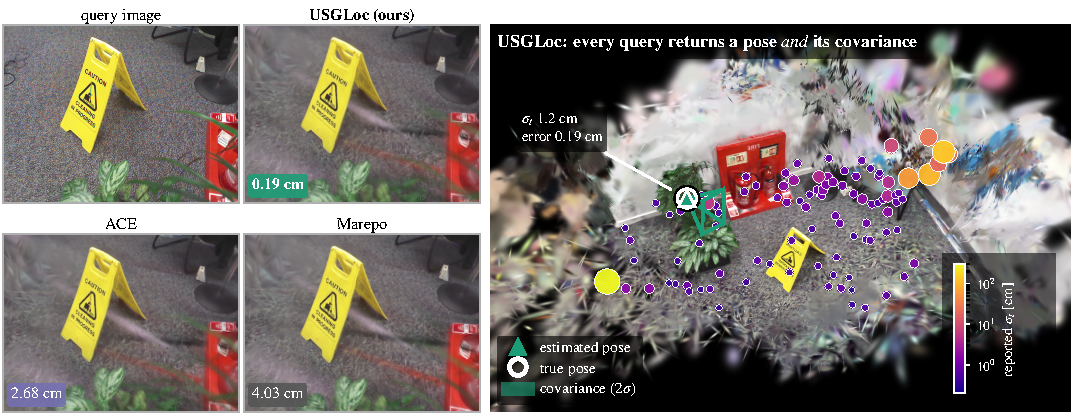
\includegraphics[width=\textwidth]{fig1_teaser.pdf}
\caption{\method{} returns a pose \emph{and} its covariance. Left: a 7-Scenes \textit{fire} query and the Gaussian map rendered at the pose each method returned, with translation error. Right: the same map from a free camera; every test query is coloured by the $\sigma_t$ \method{} reported for it, and the selected query shows its estimated pose, the true pose, and the $2\sigma$ covariance. The query is a favourable example chosen for legibility; Tables~\ref{tab:7scenes}--\ref{tab:12scenes} give the distribution.}
\label{fig:teaser}
\end{figure*}
\IEEEPARstart{V}{isual} localization estimates the 6-DoF camera pose of a query image inside a previously mapped scene, which is a core capability for indoor mobile robots and micro aerial vehicles (MAVs)~\cite{kerbl3dgs,sgloc,chukim}. On these platforms the pose is rarely consumed on its own. It enters a recursive Bayesian estimator, such as an EKF or UKF, and is fused with inertial and other cues~\cite{ukf}. This fusion is only as sound as the \emph{uncertainty} attached to each measurement. A pose without a covariance forces the estimator to assume a fixed noise model. A fixed model cannot reflect scene ambiguity, occlusion, dynamics, or texture sparsity. These are exactly the conditions under which localization degrades. An localizer should therefore output a \emph{calibrated distribution} over pose, not a point.

Classical localization is dominated by feature-based and regression-based methods. Feature-based pipelines match 2D keypoints to a 3D model and solve Perspective-$n$-Point with RANSAC~\cite{lightglue}. Absolute pose regression (APR)~\cite{posenet,marepo} and scene coordinate regression (SCR)~\cite{dsacstar,ace} learn the mapping end-to-end. 
3D Gaussian Splatting (3DGS)~\cite{kerbl3dgs} then brought high-fidelity novel-view synthesis at real-time rates. It has become an attractive map representation, and a family of 3DGS localizers now refines pose by inverting or matching against the rendered map~\cite{icomma,gsplatloc,gscpr,stdloc}. Semantics improve robustness further. SGLoc~\cite{sgloc} retrieves a coarse pose by aligning 2D and 3DGS scene-level semantic descriptors. Chu and Kim~\cite{chukim} use a language model to select ``stable'' objects for a robust submap. These methods are accurate, but they share two limitations. First, they emit a single pose and \emph{say nothing about its reliability}. Second, they handle scene dynamics implicitly or through hard, discrete object selection. Discrete selection cannot express graded confidence.

A separate line of work quantifies uncertainty rigorously, but it stops short of a calibrated pose distribution over a 3DGS map. Wu and Campbell~\cite{ksenet} learn a measurement-error \emph{distribution} for image-retrieval localization. They show that the error is non-Gaussian under hard conditions and is best modeled by a Gaussian mixture. Their setting is purely 2D, with no 3D map and no rendering. Particle-based localizers over radiance fields~\cite{locnerf} maintain a nonparametric pose belief. They report only its MAP point, without calibration. Most recently, UGS-Loc~\cite{ugsloc} guides 3DGS pose refinement with Fisher-information uncertainty maps and Monte Carlo pose sampling. It uses uncertainty only \emph{internally} and also emits a single point estimate. Evidential learning has reached scene-coordinate regression~\cite{chen2024edlscr}, but without a metric map at test time. On the mapping side, evidential semantic mapping~\cite{ebs,e2bki} propagates per-observation uncertainty with Evidential Deep Learning (EDL)~\cite{edl} and Dempster--Shafer Theory (DST)~\cite{dst}. E$^2$-BKI~\cite{e2bki} adds anisotropic Gaussian primitives and geometry-aligned kernels. Rendering-side uncertainty for radiance fields is also well studied~\cite{fisherrf}. These methods produce trustworthy \emph{maps}. Their uncertainty, however, never reaches the pose estimate that a robot consumes. To our knowledge, no existing method outputs a \emph{calibrated} pose distribution from a Gaussian-splatting map (Fig.~\ref{fig:positioning}).

\method{} fills that cell. Its design follows one principle: \emph{the map's own uncertainty should drive every stage of localization and survive to the output}. The scene is represented as an evidential semantic Gaussian map. Each object-level primitive stores geometry, an open-vocabulary CLIP~\cite{clip} embedding, and a DST belief with an explicit vacuity mass. Vacuity is the evidential measure of ignorance. It is created once, when observations are encoded, and it is never discarded. The query image is segmented~\cite{fastsam} and encoded by the \emph{same} evidential head. Query and map confidences therefore live on one scale. Every later stage is then derived as a consumer of this single signal. In the coarse stage, vacuity gates 2D--3D semantic matching, and retrieval ambiguity becomes an explicit weighted pose mixture. In the correction stage, the same vacuity gates the correspondences of a render-and-match pose correction, so geometric evidence is trusted only where the map holds semantic evidence. In the fine stage, vacuity is alpha-blended through the rasterizer exactly like color. The result is a per-pixel trust map, and moved or ambiguous content loses its vote on the pose. At the optimum, a tempered Laplace approximation turns the weighted objective into a per-hypothesis covariance. The output is a Gaussian-mixture posterior on $SE(3)$, condensed to a single Gaussian for a downstream filter. No stage requires dynamic-object heuristics or a language model. Our contributions are:

\begin{itemize}
\item \textbf{Evidential localization on a 3DGS map.} We introduce the first localizer that outputs a \emph{calibrated $SE(3)$ pose distribution} from a Gaussian-splatting map.
\item \textbf{One propagated uncertainty channel.} Every stage consumes the same evidential state. Conflict-aware DST fusion builds the map. Vacuity gates semantic matching and turns ambiguity into a weighted pose mixture, lifting the non-Gaussian error. Rendered vacuity gates the correspondences of the matching correction and weights the refinement per pixel through the standard alpha-blending kernel, replacing discrete robust-object selection with graded, evidence-driven trust.
\item \textbf{Calibrated covariance from rendering.} A Laplace approximation at the refinement optimum converts the weighted photometric objective into a per-hypothesis covariance at negligible cost. A single temperature, fitted on a held-out split, makes it honest.
\end{itemize}

\begin{figure*}[t]
\centering
\resizebox{\textwidth}{!}{% Fig. 1 -- USGLoc overview (standalone TikZ -> vector PDF).
% Compile standalone: pdflatex fig1_overview.tex
% In the paper: \resizebox{\textwidth}{!}{% Fig. 1 -- USGLoc overview (standalone TikZ -> vector PDF).
% Compile standalone: pdflatex fig1_overview.tex
% In the paper: \resizebox{\textwidth}{!}{% Fig. 1 -- USGLoc overview (standalone TikZ -> vector PDF).
% Compile standalone: pdflatex fig1_overview.tex
% In the paper: \resizebox{\textwidth}{!}{\input{figures/fig1_overview}}
%
% Design (after the STDLoc / UGS-Loc / GS-CPR / SplatHLoc figure study):
%  * slim grey OFFLINE strip (evidential mapping) on the left;
%  * Band A: the online pose flow (query -> matching -> hypotheses ->
%    refinement -> calibrated posterior);
%  * Band B: the EVIDENCE channel in gold underneath, injected upward into
%    Band A at four points (gate, correspondence gate, per-pixel weight,
%    temperature) -- the paper's thesis as the figure's macro-structure;
%  * every arrow carries an artifact glyph and a math symbol from the text;
%  * two accent colors only: gold = evidence, blue = pose distributions.
\documentclass[tikz,border=3pt]{standalone}
\usepackage{amsmath,amssymb,bm}
\usepackage{graphicx}
\usetikzlibrary{positioning,arrows.meta,backgrounds,fit,calc,shadings}

\definecolor{ink}{HTML}{273746}
\definecolor{uLow}{HTML}{1B9E77}
\definecolor{uMid}{HTML}{E6AB02}
\definecolor{uHigh}{HTML}{D95F02}
\definecolor{coarseBg}{HTML}{EAF2FB}
\definecolor{coarseLn}{HTML}{9DC3EC}
\definecolor{fineBg}{HTML}{FDF1E6}
\definecolor{fineLn}{HTML}{F0C28E}
\definecolor{encBg}{HTML}{EEF6EE}
\definecolor{encLn}{HTML}{B7D8B7}
\definecolor{outBg}{HTML}{FFF3D6}
\definecolor{outLn}{HTML}{D9A300}
\definecolor{poseC}{HTML}{2E6FAC}

\begin{document}
\begin{tikzpicture}[
  font=\footnotesize\color{ink},
  >={Stealth[length=2mm]},
  mod/.style={draw=ink!75, fill=white, rounded corners=2pt, align=center,
              minimum height=10mm, inner sep=2.5pt, line width=0.5pt},
  flow/.style={->, line width=0.7pt, draw=ink!80},
  evflow/.style={->, line width=1.0pt, draw=outLn},
  inject/.style={->, line width=1.0pt, draw=outLn, dashed},
  sym/.style={font=\scriptsize\color{ink}, inner sep=1.5pt, fill=white,
              fill opacity=0.85, text opacity=1},
  sub/.style={font=\scriptsize\color{ink!75}, align=center},
  panlab/.style={font=\scriptsize\bfseries\color{ink!80}}
]

% ============================ OFFLINE STRIP =================================
% mapping frames: three real training views
\foreach \i/\dx/\dy in {2/0.16/0.16, 1/0.08/0.08, 0/0/0}{
  \node[inner sep=0pt, draw=ink!60, line width=0.35pt]
    at (1.15+\dx, 1.42+\dy) {\includegraphics[width=10mm]{fig1_blocks/mapframe\i.png}};
}
\node[sub, anchor=north] at (1.15, 0.92) {mapping frames};
\draw[flow] (1.15, 0.72) -- (1.15, 0.12);
\node[mod, text width=23mm, font=\scriptsize\color{ink}] (edlhead) at (1.15,-0.42)
  {semantic 3DGS\\ + EDL head (3)};
\draw[flow] (1.15,-0.98) -- node[sym, right=0mm] {$(\mathbf{b},u)$} (1.15,-1.22);
% evidential map: splats colored by vacuity
% the real map, rendered from a free camera: Gaussians, not a schematic
\node[inner sep=0pt, draw=ink!60, line width=0.35pt] (map3d) at (1.15,-2.00)
  {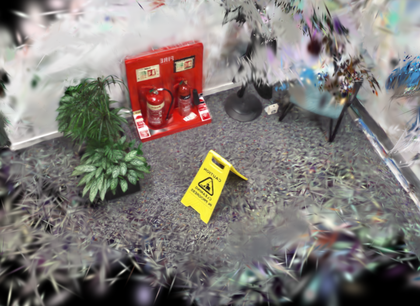
\includegraphics[width=20mm]{fig1_blocks/map3d.png}};
% vacuity key, so the colour channel carried below means something
\foreach \i/\c in {0/uLow, 1/uMid, 2/uHigh}{
  \shade[inner color=\c!25, outer color=\c!85] (0.42+0.26*\i, -3.00) circle (0.9mm);
}
\node[sub, anchor=west, font=\tiny\color{ink!75}] at (1.08,-3.00) {$u$: low$\to$high};
\node[sub, anchor=north, text width=30mm] at (1.15,-3.18)
  {evidential map $\mathcal{M}{=}\{\mathcal{G}_i\}$\\[-0.4mm]
   {\tiny $\mathcal{G}_i{=}(\bm\mu_i,\bm\Sigma_i,f_i,\mathbf{p}_i,\tilde u_i)$}};

% ============================== BAND A ======================================
% query
\node[inner sep=0pt, draw=ink!70, line width=0.5pt] (qimg) at (3.92, 1.01)
  {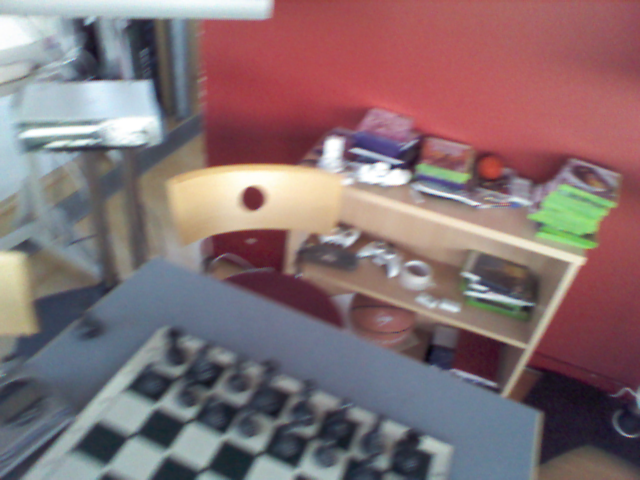
\includegraphics[width=11.5mm]{fig4/a_query.png}};
\node[sub, anchor=north] at (3.92, 0.55) {query $I_q$};

% evidential encoding
\node[mod, text width=25mm] (enc) at (6.05, 1.0)
  {Evidential\\encoding (III-B)\\{\scriptsize $\mathcal{Q}_j{=}(\mathbf{x},a,f^q,\mathbf{p}^q,u^q)$}};
\draw[flow] (4.5, 1.0) -- (enc.west);

% gated matching, with match-line glyph showing gating
\node[mod, text width=24mm, minimum height=13mm] (match) at (9.35, 1.0)
  {Vacuity-gated\\matching (III-C)};
\draw[flow] (enc.east) -- node[sym, above=0mm] {$d^q_j$} (match.west);
% match glyph below the box: two frames, kept (green) and gated-out (orange) matches
\begin{scope}[shift={(8.55, 0.28)}]
  \draw[ink!55, line width=0.4pt] (0,0) rectangle +(0.5,0.36);
  \draw[ink!55, line width=0.4pt] (1.1,0) rectangle +(0.5,0.36);
  \draw[uLow, line width=0.5pt]  (0.5,0.28) -- (1.1,0.30);
  \draw[uLow, line width=0.5pt]  (0.5,0.16) -- (1.1,0.12);
  \draw[uHigh, line width=0.5pt, dash pattern=on 1pt off 1pt] (0.5,0.05) -- (1.1,0.22);
\end{scope}

% top-k hypotheses: three fading camera frusta
\begin{scope}[shift={(12.15, 0.72)}]
  \foreach \dx/\op in {0/0.9, 0.42/0.55, 0.84/0.3}{
    \begin{scope}[shift={(\dx,0)}, opacity=\op]
      \fill[poseC!25] (0,0.66) -- (0,0.10) -- (0.5,0.38) -- cycle;
      \draw[poseC, line width=0.6pt] (0,0.66) -- (0,0.10) -- (0.5,0.38) -- cycle;
    \end{scope}
  }
\end{scope}
\node[sub, anchor=north, text width=24mm] (hyplab) at (12.85, 0.62)
  {top-$k$ hypotheses\\$\{(T^0_k,\tilde\pi_k)\}$};
\draw[flow] (match.east) -- node[sym, above=0mm] {$s_{ij}$ (6)} (12.0, 1.0);

% ---- row 2 (correction + fine + pose head), shifted under row 1 ----------
\node[mod, text width=24mm, minimum height=13mm] (corr) at (3.50, -5.80)
  {Matching\\correction (III-D)\\{\scriptsize PnP on gated matches (8)}};
\node[mod, text width=26mm, minimum height=13mm] (refine) at (6.75, -5.80)
  {Vacuity-weighted\\refinement (III-E)\\{\scriptsize $E(\bm{\xi})$ (10)}};
\node[inner sep=0pt, draw=ink!55, line width=0.4pt] (wimg) at (6.75,-7.15)
  {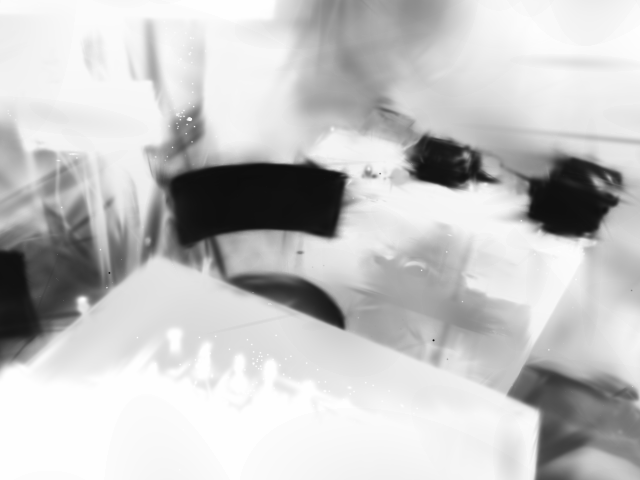
\includegraphics[width=12mm]{fig4/a_weight.png}};
\node[sub, anchor=north] at (6.75,-7.58) {per-pixel weight $w$};
\draw[flow] (corr.east) -- node[sym, above=0mm] {$T'_k$} (refine.west);

% ---- calibrated pose head ----
\node[mod, text width=21mm] (lap) at (10.15, -5.80)
  {Laplace cov.\ (11)\\{\scriptsize $\bm{\Sigma}_{\bm{\xi},k}\!\leftarrow\!\tau\hat\sigma^2(J^{\!\top}\!WJ)^{-1}$}};
\draw[flow] (refine.east) -- node[sym, above=0mm] {$\bm{\xi}^\star_k$} (lap.west);
% GMM glyph: overlapping covariance ellipses
\begin{scope}[shift={(12.55, -5.98)}]
  \draw[poseC!85, line width=0.6pt, rotate around={18:(0.32,0.28)}]
    (0.32,0.28) ellipse (4.6mm and 2.4mm);
  \draw[poseC!85, line width=0.6pt, rotate around={-12:(0.95,0.46)}]
    (0.95,0.46) ellipse (3.2mm and 1.8mm);
  \fill[poseC] (0.32,0.28) circle (0.5pt);
  \fill[poseC] (0.95,0.46) circle (0.5pt);
\end{scope}
\node[sub, anchor=north, text width=26mm] at (13.20, -6.25)
  {$p(T|I_q,\mathcal{M})$ (12)\\condense $\rightarrow$ EKF};
\draw[flow] (lap.east) -- (11.95, -5.80);

% ---- the serpentine turn: row 1 ends, row 2 begins -----------------------
\draw[flow] (13.85, 1.0) -- (14.75, 1.0) -- (14.75, -4.12)
            -- (1.30, -4.12) -- (1.30, -5.80) -- (corr.west);


% ============================== BAND B ======================================
% opinion simplex glyph
\begin{scope}[shift={(5.55,-2.65)}]
  \draw[outLn, line width=0.6pt] (0,0) -- (1.0,0) -- (0.5,0.8) -- cycle;
  \fill[outLn!45] (0.42,0.30) circle (1.6mm);
  \node[sub, anchor=north] at (0.5,-0.08) {opinion $(\mathbf{b},u)$};
\end{scope}
% DST fusion glyph: two small simplexes -> one
\begin{scope}[shift={(8.55,-2.45)}]
  \draw[outLn!70, line width=0.5pt] (0,0.12) -- (0.44,0.12) -- (0.22,0.48) -- cycle;
  \draw[outLn!70, line width=0.5pt] (0,-0.42) -- (0.44,-0.42) -- (0.22,-0.06) -- cycle;
  \node[font=\scriptsize\color{outLn}] at (0.68,-0.02) {$\oplus$};
  \draw[outLn, line width=0.6pt] (0.9,-0.28) -- (1.5,-0.28) -- (1.2,0.22) -- cycle;
  \node[sub, anchor=north, text width=24mm] at (0.26,-0.56)
    {conflict-aware fusion (4)\\[-0.3mm]{\tiny $\tilde{u}{=}\min(1,u{+}\bar\eta)$}};
\end{scope}
% vacuity heatmap glyph U_r
\node[inner sep=0pt, draw=ink!55, line width=0.4pt] (urimg) at (10.95,-2.34)
  {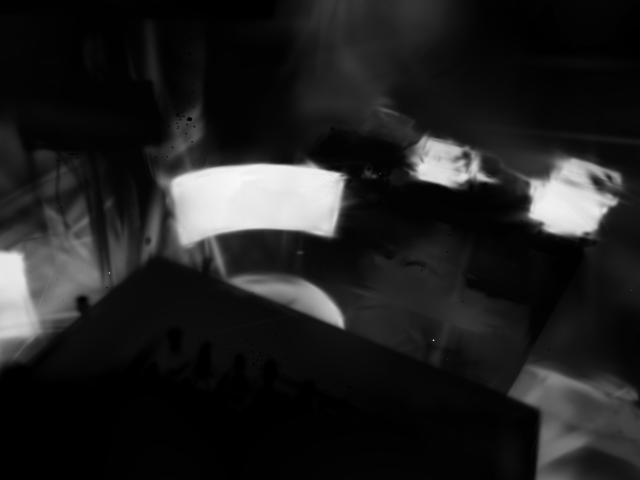
\includegraphics[width=12mm]{fig4/a_vacuity.png}};
\node[sub, anchor=north] at (11.05,-2.90) {rendered $U_r$ (9)};
% temperature chip
\node[mod, draw=outLn, text width=16mm, font=\scriptsize\color{ink}] (temp) at (13.35,-2.45)
  {temperature $\tau$\\(held-out fit)};

% the gold evidence rail
\draw[evflow] (2.1,-2.1) -- node[sym, above=0mm] {$u$} (5.45,-2.35);
\draw[evflow] (6.75,-2.35) -- (8.4,-2.5);
\draw[evflow] (9.95,-2.34) -- node[sym, above=0.6mm, pos=0.45] {$\tilde{u}_i$ per splat} (urimg.west);
\draw[evflow] (urimg.east) -- (temp.west);

% injections: UP into row 1, DOWN into row 2 -- one channel, both bands
\draw[inject] (9.35,-1.95) -- node[sym, right=0.2mm]
  {gate $e^{-\lambda_u(\tilde{u}^G_i+u^q_j)}$} (match.south);
\draw[inject] (10.25,-3.60) -- node[sym, left=0.2mm, pos=0.42, fill=white, inner sep=1pt]
  {$\bar U_r{\le}u_{\max}$} (corr.north);
\draw[inject] (11.65,-3.60) -- node[sym, right=0.2mm, pos=0.42, fill=white, inner sep=1pt]
  {$w{=}e^{-\gamma U_r}$} (refine.north);
\draw[inject] (temp.south) -- node[sym, right=0.2mm] {$\tau$} (lap.north);

% ======================= PANELS (background layer) ==========================
\begin{scope}[on background layer]
  % offline strip
  \node[fill=ink!5, draw=ink!35, dashed, rounded corners=3pt, inner sep=2.6mm,
        fit={(edlhead) (map3d) (-0.20,2.05) (2.55,-3.95)}] (offpan) {};
  % coarse panel
  \node[fill=coarseBg, draw=coarseLn, rounded corners=3pt, inner sep=2.8mm,
        fit={(enc) (match) (hyplab) (13.9,0.2)}] (cpan) {};
  % fine panel
  \node[fill=fineBg, draw=fineLn, rounded corners=3pt, inner sep=2.8mm,
        fit={(corr) (refine) (wimg) (6.75,-7.75)}] (fpan) {};
  % calibrated pose head panel
  \node[fill=poseC!8, draw=poseC!60, rounded corners=3pt, inner sep=2.8mm,
        fit={(lap) (14.6,-6.45) (14.6,-5.25)}] (ppan) {};
  % evidence band
  \node[fill=outBg, draw=outLn!70, rounded corners=3pt, inner sep=2.8mm,
        fit={(5.45,-1.8) (temp) (urimg) (14.3,-3.42) (5.45,-3.42)}] (epan) {};
\end{scope}
\node[panlab, anchor=south west] at (offpan.north west)
  {Offline: evidential mapping (III-A)};
\node[panlab, anchor=south west] at (cpan.north west) {Coarse (IV-B,C)};
\node[panlab, anchor=south west] at (fpan.north west) {Correction + fine (IV-D,E)};
\node[panlab, anchor=south west, color=poseC] at (ppan.north west)
  {Calibrated pose posterior};
\node[panlab, anchor=south west, color=outLn!80!ink] at (epan.north west)
  {One evidential channel: created once, never dropped};

% map feeds the online flow
\draw[flow] (2.18,-0.42) -- node[sym, above=0.4mm, pos=0.62] {$\mathcal{M}$}
  (2.95,-0.42) -- (8.4,-0.42) -- (match.south west);

\end{tikzpicture}
\end{document}
}
%
% Design (after the STDLoc / UGS-Loc / GS-CPR / SplatHLoc figure study):
%  * slim grey OFFLINE strip (evidential mapping) on the left;
%  * Band A: the online pose flow (query -> matching -> hypotheses ->
%    refinement -> calibrated posterior);
%  * Band B: the EVIDENCE channel in gold underneath, injected upward into
%    Band A at four points (gate, correspondence gate, per-pixel weight,
%    temperature) -- the paper's thesis as the figure's macro-structure;
%  * every arrow carries an artifact glyph and a math symbol from the text;
%  * two accent colors only: gold = evidence, blue = pose distributions.
\documentclass[tikz,border=3pt]{standalone}
\usepackage{amsmath,amssymb,bm}
\usepackage{graphicx}
\usetikzlibrary{positioning,arrows.meta,backgrounds,fit,calc,shadings}

\definecolor{ink}{HTML}{273746}
\definecolor{uLow}{HTML}{1B9E77}
\definecolor{uMid}{HTML}{E6AB02}
\definecolor{uHigh}{HTML}{D95F02}
\definecolor{coarseBg}{HTML}{EAF2FB}
\definecolor{coarseLn}{HTML}{9DC3EC}
\definecolor{fineBg}{HTML}{FDF1E6}
\definecolor{fineLn}{HTML}{F0C28E}
\definecolor{encBg}{HTML}{EEF6EE}
\definecolor{encLn}{HTML}{B7D8B7}
\definecolor{outBg}{HTML}{FFF3D6}
\definecolor{outLn}{HTML}{D9A300}
\definecolor{poseC}{HTML}{2E6FAC}

\begin{document}
\begin{tikzpicture}[
  font=\footnotesize\color{ink},
  >={Stealth[length=2mm]},
  mod/.style={draw=ink!75, fill=white, rounded corners=2pt, align=center,
              minimum height=10mm, inner sep=2.5pt, line width=0.5pt},
  flow/.style={->, line width=0.7pt, draw=ink!80},
  evflow/.style={->, line width=1.0pt, draw=outLn},
  inject/.style={->, line width=1.0pt, draw=outLn, dashed},
  sym/.style={font=\scriptsize\color{ink}, inner sep=1.5pt, fill=white,
              fill opacity=0.85, text opacity=1},
  sub/.style={font=\scriptsize\color{ink!75}, align=center},
  panlab/.style={font=\scriptsize\bfseries\color{ink!80}}
]

% ============================ OFFLINE STRIP =================================
% mapping frames: three real training views
\foreach \i/\dx/\dy in {2/0.16/0.16, 1/0.08/0.08, 0/0/0}{
  \node[inner sep=0pt, draw=ink!60, line width=0.35pt]
    at (1.15+\dx, 1.42+\dy) {\includegraphics[width=10mm]{fig1_blocks/mapframe\i.png}};
}
\node[sub, anchor=north] at (1.15, 0.92) {mapping frames};
\draw[flow] (1.15, 0.72) -- (1.15, 0.12);
\node[mod, text width=23mm, font=\scriptsize\color{ink}] (edlhead) at (1.15,-0.42)
  {semantic 3DGS\\ + EDL head (3)};
\draw[flow] (1.15,-0.98) -- node[sym, right=0mm] {$(\mathbf{b},u)$} (1.15,-1.22);
% evidential map: splats colored by vacuity
% the real map, rendered from a free camera: Gaussians, not a schematic
\node[inner sep=0pt, draw=ink!60, line width=0.35pt] (map3d) at (1.15,-2.00)
  {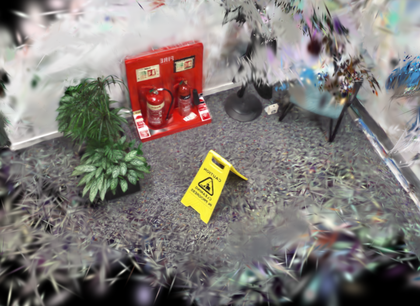
\includegraphics[width=20mm]{fig1_blocks/map3d.png}};
% vacuity key, so the colour channel carried below means something
\foreach \i/\c in {0/uLow, 1/uMid, 2/uHigh}{
  \shade[inner color=\c!25, outer color=\c!85] (0.42+0.26*\i, -3.00) circle (0.9mm);
}
\node[sub, anchor=west, font=\tiny\color{ink!75}] at (1.08,-3.00) {$u$: low$\to$high};
\node[sub, anchor=north, text width=30mm] at (1.15,-3.18)
  {evidential map $\mathcal{M}{=}\{\mathcal{G}_i\}$\\[-0.4mm]
   {\tiny $\mathcal{G}_i{=}(\bm\mu_i,\bm\Sigma_i,f_i,\mathbf{p}_i,\tilde u_i)$}};

% ============================== BAND A ======================================
% query
\node[inner sep=0pt, draw=ink!70, line width=0.5pt] (qimg) at (3.92, 1.01)
  {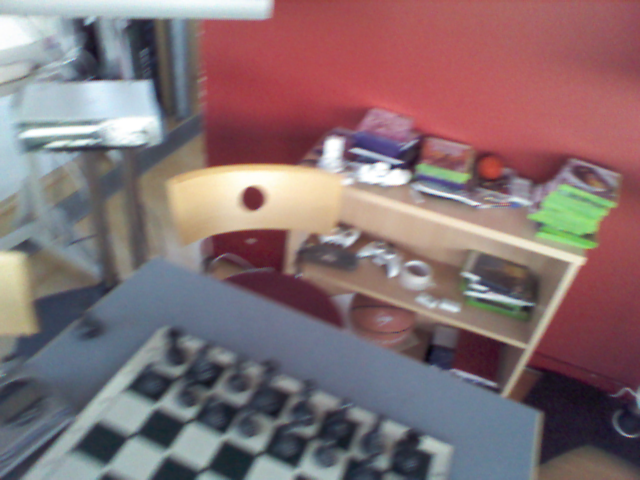
\includegraphics[width=11.5mm]{fig4/a_query.png}};
\node[sub, anchor=north] at (3.92, 0.55) {query $I_q$};

% evidential encoding
\node[mod, text width=25mm] (enc) at (6.05, 1.0)
  {Evidential\\encoding (III-B)\\{\scriptsize $\mathcal{Q}_j{=}(\mathbf{x},a,f^q,\mathbf{p}^q,u^q)$}};
\draw[flow] (4.5, 1.0) -- (enc.west);

% gated matching, with match-line glyph showing gating
\node[mod, text width=24mm, minimum height=13mm] (match) at (9.35, 1.0)
  {Vacuity-gated\\matching (III-C)};
\draw[flow] (enc.east) -- node[sym, above=0mm] {$d^q_j$} (match.west);
% match glyph below the box: two frames, kept (green) and gated-out (orange) matches
\begin{scope}[shift={(8.55, 0.28)}]
  \draw[ink!55, line width=0.4pt] (0,0) rectangle +(0.5,0.36);
  \draw[ink!55, line width=0.4pt] (1.1,0) rectangle +(0.5,0.36);
  \draw[uLow, line width=0.5pt]  (0.5,0.28) -- (1.1,0.30);
  \draw[uLow, line width=0.5pt]  (0.5,0.16) -- (1.1,0.12);
  \draw[uHigh, line width=0.5pt, dash pattern=on 1pt off 1pt] (0.5,0.05) -- (1.1,0.22);
\end{scope}

% top-k hypotheses: three fading camera frusta
\begin{scope}[shift={(12.15, 0.72)}]
  \foreach \dx/\op in {0/0.9, 0.42/0.55, 0.84/0.3}{
    \begin{scope}[shift={(\dx,0)}, opacity=\op]
      \fill[poseC!25] (0,0.66) -- (0,0.10) -- (0.5,0.38) -- cycle;
      \draw[poseC, line width=0.6pt] (0,0.66) -- (0,0.10) -- (0.5,0.38) -- cycle;
    \end{scope}
  }
\end{scope}
\node[sub, anchor=north, text width=24mm] (hyplab) at (12.85, 0.62)
  {top-$k$ hypotheses\\$\{(T^0_k,\tilde\pi_k)\}$};
\draw[flow] (match.east) -- node[sym, above=0mm] {$s_{ij}$ (6)} (12.0, 1.0);

% ---- row 2 (correction + fine + pose head), shifted under row 1 ----------
\node[mod, text width=24mm, minimum height=13mm] (corr) at (3.50, -5.80)
  {Matching\\correction (III-D)\\{\scriptsize PnP on gated matches (8)}};
\node[mod, text width=26mm, minimum height=13mm] (refine) at (6.75, -5.80)
  {Vacuity-weighted\\refinement (III-E)\\{\scriptsize $E(\bm{\xi})$ (10)}};
\node[inner sep=0pt, draw=ink!55, line width=0.4pt] (wimg) at (6.75,-7.15)
  {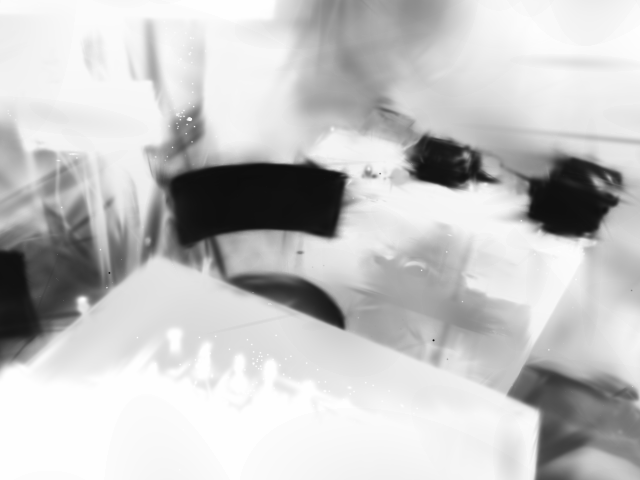
\includegraphics[width=12mm]{fig4/a_weight.png}};
\node[sub, anchor=north] at (6.75,-7.58) {per-pixel weight $w$};
\draw[flow] (corr.east) -- node[sym, above=0mm] {$T'_k$} (refine.west);

% ---- calibrated pose head ----
\node[mod, text width=21mm] (lap) at (10.15, -5.80)
  {Laplace cov.\ (11)\\{\scriptsize $\bm{\Sigma}_{\bm{\xi},k}\!\leftarrow\!\tau\hat\sigma^2(J^{\!\top}\!WJ)^{-1}$}};
\draw[flow] (refine.east) -- node[sym, above=0mm] {$\bm{\xi}^\star_k$} (lap.west);
% GMM glyph: overlapping covariance ellipses
\begin{scope}[shift={(12.55, -5.98)}]
  \draw[poseC!85, line width=0.6pt, rotate around={18:(0.32,0.28)}]
    (0.32,0.28) ellipse (4.6mm and 2.4mm);
  \draw[poseC!85, line width=0.6pt, rotate around={-12:(0.95,0.46)}]
    (0.95,0.46) ellipse (3.2mm and 1.8mm);
  \fill[poseC] (0.32,0.28) circle (0.5pt);
  \fill[poseC] (0.95,0.46) circle (0.5pt);
\end{scope}
\node[sub, anchor=north, text width=26mm] at (13.20, -6.25)
  {$p(T|I_q,\mathcal{M})$ (12)\\condense $\rightarrow$ EKF};
\draw[flow] (lap.east) -- (11.95, -5.80);

% ---- the serpentine turn: row 1 ends, row 2 begins -----------------------
\draw[flow] (13.85, 1.0) -- (14.75, 1.0) -- (14.75, -4.12)
            -- (1.30, -4.12) -- (1.30, -5.80) -- (corr.west);


% ============================== BAND B ======================================
% opinion simplex glyph
\begin{scope}[shift={(5.55,-2.65)}]
  \draw[outLn, line width=0.6pt] (0,0) -- (1.0,0) -- (0.5,0.8) -- cycle;
  \fill[outLn!45] (0.42,0.30) circle (1.6mm);
  \node[sub, anchor=north] at (0.5,-0.08) {opinion $(\mathbf{b},u)$};
\end{scope}
% DST fusion glyph: two small simplexes -> one
\begin{scope}[shift={(8.55,-2.45)}]
  \draw[outLn!70, line width=0.5pt] (0,0.12) -- (0.44,0.12) -- (0.22,0.48) -- cycle;
  \draw[outLn!70, line width=0.5pt] (0,-0.42) -- (0.44,-0.42) -- (0.22,-0.06) -- cycle;
  \node[font=\scriptsize\color{outLn}] at (0.68,-0.02) {$\oplus$};
  \draw[outLn, line width=0.6pt] (0.9,-0.28) -- (1.5,-0.28) -- (1.2,0.22) -- cycle;
  \node[sub, anchor=north, text width=24mm] at (0.26,-0.56)
    {conflict-aware fusion (4)\\[-0.3mm]{\tiny $\tilde{u}{=}\min(1,u{+}\bar\eta)$}};
\end{scope}
% vacuity heatmap glyph U_r
\node[inner sep=0pt, draw=ink!55, line width=0.4pt] (urimg) at (10.95,-2.34)
  {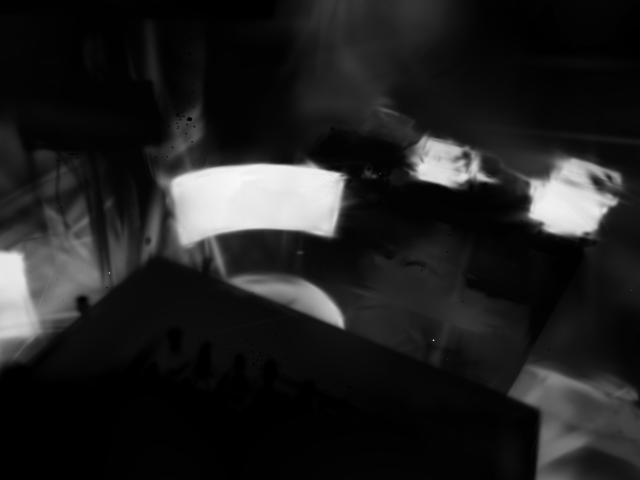
\includegraphics[width=12mm]{fig4/a_vacuity.png}};
\node[sub, anchor=north] at (11.05,-2.90) {rendered $U_r$ (9)};
% temperature chip
\node[mod, draw=outLn, text width=16mm, font=\scriptsize\color{ink}] (temp) at (13.35,-2.45)
  {temperature $\tau$\\(held-out fit)};

% the gold evidence rail
\draw[evflow] (2.1,-2.1) -- node[sym, above=0mm] {$u$} (5.45,-2.35);
\draw[evflow] (6.75,-2.35) -- (8.4,-2.5);
\draw[evflow] (9.95,-2.34) -- node[sym, above=0.6mm, pos=0.45] {$\tilde{u}_i$ per splat} (urimg.west);
\draw[evflow] (urimg.east) -- (temp.west);

% injections: UP into row 1, DOWN into row 2 -- one channel, both bands
\draw[inject] (9.35,-1.95) -- node[sym, right=0.2mm]
  {gate $e^{-\lambda_u(\tilde{u}^G_i+u^q_j)}$} (match.south);
\draw[inject] (10.25,-3.60) -- node[sym, left=0.2mm, pos=0.42, fill=white, inner sep=1pt]
  {$\bar U_r{\le}u_{\max}$} (corr.north);
\draw[inject] (11.65,-3.60) -- node[sym, right=0.2mm, pos=0.42, fill=white, inner sep=1pt]
  {$w{=}e^{-\gamma U_r}$} (refine.north);
\draw[inject] (temp.south) -- node[sym, right=0.2mm] {$\tau$} (lap.north);

% ======================= PANELS (background layer) ==========================
\begin{scope}[on background layer]
  % offline strip
  \node[fill=ink!5, draw=ink!35, dashed, rounded corners=3pt, inner sep=2.6mm,
        fit={(edlhead) (map3d) (-0.20,2.05) (2.55,-3.95)}] (offpan) {};
  % coarse panel
  \node[fill=coarseBg, draw=coarseLn, rounded corners=3pt, inner sep=2.8mm,
        fit={(enc) (match) (hyplab) (13.9,0.2)}] (cpan) {};
  % fine panel
  \node[fill=fineBg, draw=fineLn, rounded corners=3pt, inner sep=2.8mm,
        fit={(corr) (refine) (wimg) (6.75,-7.75)}] (fpan) {};
  % calibrated pose head panel
  \node[fill=poseC!8, draw=poseC!60, rounded corners=3pt, inner sep=2.8mm,
        fit={(lap) (14.6,-6.45) (14.6,-5.25)}] (ppan) {};
  % evidence band
  \node[fill=outBg, draw=outLn!70, rounded corners=3pt, inner sep=2.8mm,
        fit={(5.45,-1.8) (temp) (urimg) (14.3,-3.42) (5.45,-3.42)}] (epan) {};
\end{scope}
\node[panlab, anchor=south west] at (offpan.north west)
  {Offline: evidential mapping (III-A)};
\node[panlab, anchor=south west] at (cpan.north west) {Coarse (IV-B,C)};
\node[panlab, anchor=south west] at (fpan.north west) {Correction + fine (IV-D,E)};
\node[panlab, anchor=south west, color=poseC] at (ppan.north west)
  {Calibrated pose posterior};
\node[panlab, anchor=south west, color=outLn!80!ink] at (epan.north west)
  {One evidential channel: created once, never dropped};

% map feeds the online flow
\draw[flow] (2.18,-0.42) -- node[sym, above=0.4mm, pos=0.62] {$\mathcal{M}$}
  (2.95,-0.42) -- (8.4,-0.42) -- (match.south west);

\end{tikzpicture}
\end{document}
}
%
% Design (after the STDLoc / UGS-Loc / GS-CPR / SplatHLoc figure study):
%  * slim grey OFFLINE strip (evidential mapping) on the left;
%  * Band A: the online pose flow (query -> matching -> hypotheses ->
%    refinement -> calibrated posterior);
%  * Band B: the EVIDENCE channel in gold underneath, injected upward into
%    Band A at four points (gate, correspondence gate, per-pixel weight,
%    temperature) -- the paper's thesis as the figure's macro-structure;
%  * every arrow carries an artifact glyph and a math symbol from the text;
%  * two accent colors only: gold = evidence, blue = pose distributions.
\documentclass[tikz,border=3pt]{standalone}
\usepackage{amsmath,amssymb,bm}
\usepackage{graphicx}
\usetikzlibrary{positioning,arrows.meta,backgrounds,fit,calc,shadings}

\definecolor{ink}{HTML}{273746}
\definecolor{uLow}{HTML}{1B9E77}
\definecolor{uMid}{HTML}{E6AB02}
\definecolor{uHigh}{HTML}{D95F02}
\definecolor{coarseBg}{HTML}{EAF2FB}
\definecolor{coarseLn}{HTML}{9DC3EC}
\definecolor{fineBg}{HTML}{FDF1E6}
\definecolor{fineLn}{HTML}{F0C28E}
\definecolor{encBg}{HTML}{EEF6EE}
\definecolor{encLn}{HTML}{B7D8B7}
\definecolor{outBg}{HTML}{FFF3D6}
\definecolor{outLn}{HTML}{D9A300}
\definecolor{poseC}{HTML}{2E6FAC}

\begin{document}
\begin{tikzpicture}[
  font=\footnotesize\color{ink},
  >={Stealth[length=2mm]},
  mod/.style={draw=ink!75, fill=white, rounded corners=2pt, align=center,
              minimum height=10mm, inner sep=2.5pt, line width=0.5pt},
  flow/.style={->, line width=0.7pt, draw=ink!80},
  evflow/.style={->, line width=1.0pt, draw=outLn},
  inject/.style={->, line width=1.0pt, draw=outLn, dashed},
  sym/.style={font=\scriptsize\color{ink}, inner sep=1.5pt, fill=white,
              fill opacity=0.85, text opacity=1},
  sub/.style={font=\scriptsize\color{ink!75}, align=center},
  panlab/.style={font=\scriptsize\bfseries\color{ink!80}}
]

% ============================ OFFLINE STRIP =================================
% mapping frames: three real training views
\foreach \i/\dx/\dy in {2/0.16/0.16, 1/0.08/0.08, 0/0/0}{
  \node[inner sep=0pt, draw=ink!60, line width=0.35pt]
    at (1.15+\dx, 1.42+\dy) {\includegraphics[width=10mm]{fig1_blocks/mapframe\i.png}};
}
\node[sub, anchor=north] at (1.15, 0.92) {mapping frames};
\draw[flow] (1.15, 0.72) -- (1.15, 0.12);
\node[mod, text width=23mm, font=\scriptsize\color{ink}] (edlhead) at (1.15,-0.42)
  {semantic 3DGS\\ + EDL head (3)};
\draw[flow] (1.15,-0.98) -- node[sym, right=0mm] {$(\mathbf{b},u)$} (1.15,-1.22);
% evidential map: splats colored by vacuity
% the real map, rendered from a free camera: Gaussians, not a schematic
\node[inner sep=0pt, draw=ink!60, line width=0.35pt] (map3d) at (1.15,-2.00)
  {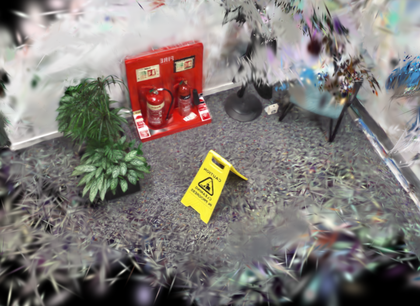
\includegraphics[width=20mm]{fig1_blocks/map3d.png}};
% vacuity key, so the colour channel carried below means something
\foreach \i/\c in {0/uLow, 1/uMid, 2/uHigh}{
  \shade[inner color=\c!25, outer color=\c!85] (0.42+0.26*\i, -3.00) circle (0.9mm);
}
\node[sub, anchor=west, font=\tiny\color{ink!75}] at (1.08,-3.00) {$u$: low$\to$high};
\node[sub, anchor=north, text width=30mm] at (1.15,-3.18)
  {evidential map $\mathcal{M}{=}\{\mathcal{G}_i\}$\\[-0.4mm]
   {\tiny $\mathcal{G}_i{=}(\bm\mu_i,\bm\Sigma_i,f_i,\mathbf{p}_i,\tilde u_i)$}};

% ============================== BAND A ======================================
% query
\node[inner sep=0pt, draw=ink!70, line width=0.5pt] (qimg) at (3.92, 1.01)
  {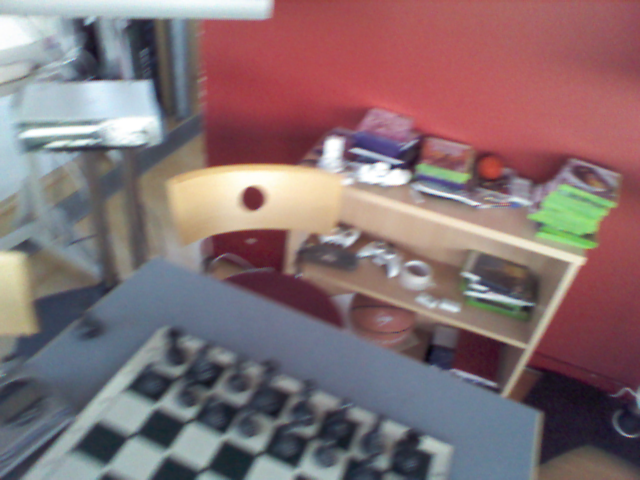
\includegraphics[width=11.5mm]{fig4/a_query.png}};
\node[sub, anchor=north] at (3.92, 0.55) {query $I_q$};

% evidential encoding
\node[mod, text width=25mm] (enc) at (6.05, 1.0)
  {Evidential\\encoding (III-B)\\{\scriptsize $\mathcal{Q}_j{=}(\mathbf{x},a,f^q,\mathbf{p}^q,u^q)$}};
\draw[flow] (4.5, 1.0) -- (enc.west);

% gated matching, with match-line glyph showing gating
\node[mod, text width=24mm, minimum height=13mm] (match) at (9.35, 1.0)
  {Vacuity-gated\\matching (III-C)};
\draw[flow] (enc.east) -- node[sym, above=0mm] {$d^q_j$} (match.west);
% match glyph below the box: two frames, kept (green) and gated-out (orange) matches
\begin{scope}[shift={(8.55, 0.28)}]
  \draw[ink!55, line width=0.4pt] (0,0) rectangle +(0.5,0.36);
  \draw[ink!55, line width=0.4pt] (1.1,0) rectangle +(0.5,0.36);
  \draw[uLow, line width=0.5pt]  (0.5,0.28) -- (1.1,0.30);
  \draw[uLow, line width=0.5pt]  (0.5,0.16) -- (1.1,0.12);
  \draw[uHigh, line width=0.5pt, dash pattern=on 1pt off 1pt] (0.5,0.05) -- (1.1,0.22);
\end{scope}

% top-k hypotheses: three fading camera frusta
\begin{scope}[shift={(12.15, 0.72)}]
  \foreach \dx/\op in {0/0.9, 0.42/0.55, 0.84/0.3}{
    \begin{scope}[shift={(\dx,0)}, opacity=\op]
      \fill[poseC!25] (0,0.66) -- (0,0.10) -- (0.5,0.38) -- cycle;
      \draw[poseC, line width=0.6pt] (0,0.66) -- (0,0.10) -- (0.5,0.38) -- cycle;
    \end{scope}
  }
\end{scope}
\node[sub, anchor=north, text width=24mm] (hyplab) at (12.85, 0.62)
  {top-$k$ hypotheses\\$\{(T^0_k,\tilde\pi_k)\}$};
\draw[flow] (match.east) -- node[sym, above=0mm] {$s_{ij}$ (6)} (12.0, 1.0);

% ---- row 2 (correction + fine + pose head), shifted under row 1 ----------
\node[mod, text width=24mm, minimum height=13mm] (corr) at (3.50, -5.80)
  {Matching\\correction (III-D)\\{\scriptsize PnP on gated matches (8)}};
\node[mod, text width=26mm, minimum height=13mm] (refine) at (6.75, -5.80)
  {Vacuity-weighted\\refinement (III-E)\\{\scriptsize $E(\bm{\xi})$ (10)}};
\node[inner sep=0pt, draw=ink!55, line width=0.4pt] (wimg) at (6.75,-7.15)
  {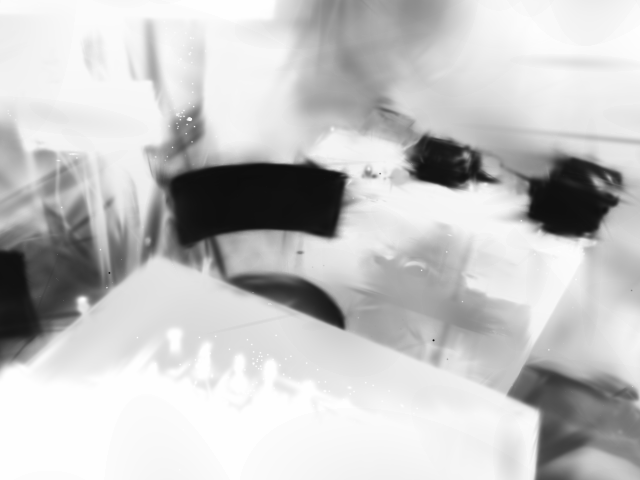
\includegraphics[width=12mm]{fig4/a_weight.png}};
\node[sub, anchor=north] at (6.75,-7.58) {per-pixel weight $w$};
\draw[flow] (corr.east) -- node[sym, above=0mm] {$T'_k$} (refine.west);

% ---- calibrated pose head ----
\node[mod, text width=21mm] (lap) at (10.15, -5.80)
  {Laplace cov.\ (11)\\{\scriptsize $\bm{\Sigma}_{\bm{\xi},k}\!\leftarrow\!\tau\hat\sigma^2(J^{\!\top}\!WJ)^{-1}$}};
\draw[flow] (refine.east) -- node[sym, above=0mm] {$\bm{\xi}^\star_k$} (lap.west);
% GMM glyph: overlapping covariance ellipses
\begin{scope}[shift={(12.55, -5.98)}]
  \draw[poseC!85, line width=0.6pt, rotate around={18:(0.32,0.28)}]
    (0.32,0.28) ellipse (4.6mm and 2.4mm);
  \draw[poseC!85, line width=0.6pt, rotate around={-12:(0.95,0.46)}]
    (0.95,0.46) ellipse (3.2mm and 1.8mm);
  \fill[poseC] (0.32,0.28) circle (0.5pt);
  \fill[poseC] (0.95,0.46) circle (0.5pt);
\end{scope}
\node[sub, anchor=north, text width=26mm] at (13.20, -6.25)
  {$p(T|I_q,\mathcal{M})$ (12)\\condense $\rightarrow$ EKF};
\draw[flow] (lap.east) -- (11.95, -5.80);

% ---- the serpentine turn: row 1 ends, row 2 begins -----------------------
\draw[flow] (13.85, 1.0) -- (14.75, 1.0) -- (14.75, -4.12)
            -- (1.30, -4.12) -- (1.30, -5.80) -- (corr.west);


% ============================== BAND B ======================================
% opinion simplex glyph
\begin{scope}[shift={(5.55,-2.65)}]
  \draw[outLn, line width=0.6pt] (0,0) -- (1.0,0) -- (0.5,0.8) -- cycle;
  \fill[outLn!45] (0.42,0.30) circle (1.6mm);
  \node[sub, anchor=north] at (0.5,-0.08) {opinion $(\mathbf{b},u)$};
\end{scope}
% DST fusion glyph: two small simplexes -> one
\begin{scope}[shift={(8.55,-2.45)}]
  \draw[outLn!70, line width=0.5pt] (0,0.12) -- (0.44,0.12) -- (0.22,0.48) -- cycle;
  \draw[outLn!70, line width=0.5pt] (0,-0.42) -- (0.44,-0.42) -- (0.22,-0.06) -- cycle;
  \node[font=\scriptsize\color{outLn}] at (0.68,-0.02) {$\oplus$};
  \draw[outLn, line width=0.6pt] (0.9,-0.28) -- (1.5,-0.28) -- (1.2,0.22) -- cycle;
  \node[sub, anchor=north, text width=24mm] at (0.26,-0.56)
    {conflict-aware fusion (4)\\[-0.3mm]{\tiny $\tilde{u}{=}\min(1,u{+}\bar\eta)$}};
\end{scope}
% vacuity heatmap glyph U_r
\node[inner sep=0pt, draw=ink!55, line width=0.4pt] (urimg) at (10.95,-2.34)
  {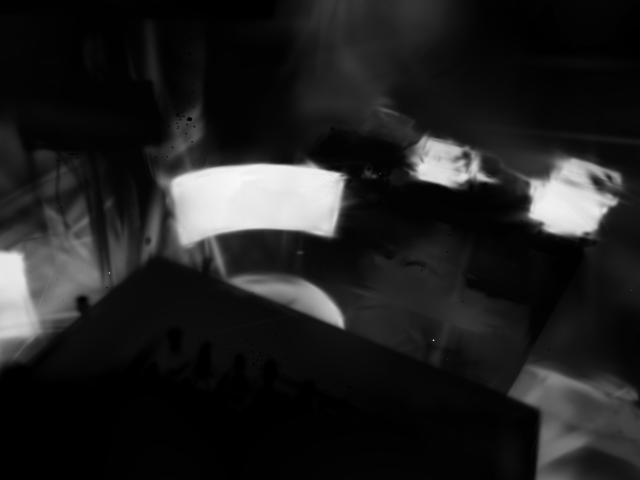
\includegraphics[width=12mm]{fig4/a_vacuity.png}};
\node[sub, anchor=north] at (11.05,-2.90) {rendered $U_r$ (9)};
% temperature chip
\node[mod, draw=outLn, text width=16mm, font=\scriptsize\color{ink}] (temp) at (13.35,-2.45)
  {temperature $\tau$\\(held-out fit)};

% the gold evidence rail
\draw[evflow] (2.1,-2.1) -- node[sym, above=0mm] {$u$} (5.45,-2.35);
\draw[evflow] (6.75,-2.35) -- (8.4,-2.5);
\draw[evflow] (9.95,-2.34) -- node[sym, above=0.6mm, pos=0.45] {$\tilde{u}_i$ per splat} (urimg.west);
\draw[evflow] (urimg.east) -- (temp.west);

% injections: UP into row 1, DOWN into row 2 -- one channel, both bands
\draw[inject] (9.35,-1.95) -- node[sym, right=0.2mm]
  {gate $e^{-\lambda_u(\tilde{u}^G_i+u^q_j)}$} (match.south);
\draw[inject] (10.25,-3.60) -- node[sym, left=0.2mm, pos=0.42, fill=white, inner sep=1pt]
  {$\bar U_r{\le}u_{\max}$} (corr.north);
\draw[inject] (11.65,-3.60) -- node[sym, right=0.2mm, pos=0.42, fill=white, inner sep=1pt]
  {$w{=}e^{-\gamma U_r}$} (refine.north);
\draw[inject] (temp.south) -- node[sym, right=0.2mm] {$\tau$} (lap.north);

% ======================= PANELS (background layer) ==========================
\begin{scope}[on background layer]
  % offline strip
  \node[fill=ink!5, draw=ink!35, dashed, rounded corners=3pt, inner sep=2.6mm,
        fit={(edlhead) (map3d) (-0.20,2.05) (2.55,-3.95)}] (offpan) {};
  % coarse panel
  \node[fill=coarseBg, draw=coarseLn, rounded corners=3pt, inner sep=2.8mm,
        fit={(enc) (match) (hyplab) (13.9,0.2)}] (cpan) {};
  % fine panel
  \node[fill=fineBg, draw=fineLn, rounded corners=3pt, inner sep=2.8mm,
        fit={(corr) (refine) (wimg) (6.75,-7.75)}] (fpan) {};
  % calibrated pose head panel
  \node[fill=poseC!8, draw=poseC!60, rounded corners=3pt, inner sep=2.8mm,
        fit={(lap) (14.6,-6.45) (14.6,-5.25)}] (ppan) {};
  % evidence band
  \node[fill=outBg, draw=outLn!70, rounded corners=3pt, inner sep=2.8mm,
        fit={(5.45,-1.8) (temp) (urimg) (14.3,-3.42) (5.45,-3.42)}] (epan) {};
\end{scope}
\node[panlab, anchor=south west] at (offpan.north west)
  {Offline: evidential mapping (III-A)};
\node[panlab, anchor=south west] at (cpan.north west) {Coarse (IV-B,C)};
\node[panlab, anchor=south west] at (fpan.north west) {Correction + fine (IV-D,E)};
\node[panlab, anchor=south west, color=poseC] at (ppan.north west)
  {Calibrated pose posterior};
\node[panlab, anchor=south west, color=outLn!80!ink] at (epan.north west)
  {One evidential channel: created once, never dropped};

% map feeds the online flow
\draw[flow] (2.18,-0.42) -- node[sym, above=0.4mm, pos=0.62] {$\mathcal{M}$}
  (2.95,-0.42) -- (8.4,-0.42) -- (match.south west);

\end{tikzpicture}
\end{document}
}
\caption{Overview of \method{}. \textbf{Offline} (left, grey): mapping frames train a semantic 3DGS map with an EDL head. Conflict-aware DST fusion turns per-observation opinions $(\mathbf{b},u)$ into evidential primitives $\mathcal{G}_i=(\bm\mu_i,\bm\Sigma_i,f_i,\mathbf{p}_i,\tilde{u}_i)$. \textbf{Online} (top): the query is encoded by the same evidential head, matched against the map, and refined by differentiable rendering. The result is a calibrated Gaussian-mixture posterior $p(T\,|\,I_q,\mathcal{M})$ that condenses to a single Gaussian for an EKF. \textbf{One evidential channel} (bottom, gold): the same vacuity signal is injected at four points. It gates matching, it gates the correspondences of the matching correction, it weights the rendering residual per pixel, and it scales the Laplace covariance through the held-out temperature $\tau$. Equation numbers in parentheses.}
\label{fig:overview}
\end{figure*}

%==============================================================================
\section{Related Work}

\begin{figure}[t]
\centering
\resizebox{0.95\columnwidth}{!}{% Fig. 2 -- Positioning of USGLoc in the design space (standalone TikZ).
% Compile: pdflatex fig2_positioning.tex  ->  fig2_positioning.pdf
% In the paper: \includegraphics[width=\columnwidth]{fig2_positioning.pdf}
\documentclass[tikz,border=3pt]{standalone}
\usepackage{amsmath,amssymb}
\usetikzlibrary{positioning}

\definecolor{ink}{HTML}{273746}
\definecolor{mapprin}{HTML}{E8F4EF}
\definecolor{mappt}{HTML}{F2F3F4}
\definecolor{locpt}{HTML}{EAF2FB}
\definecolor{ourstr}{HTML}{FFF3D6}
\definecolor{outLn}{HTML}{D9A300}

\begin{document}
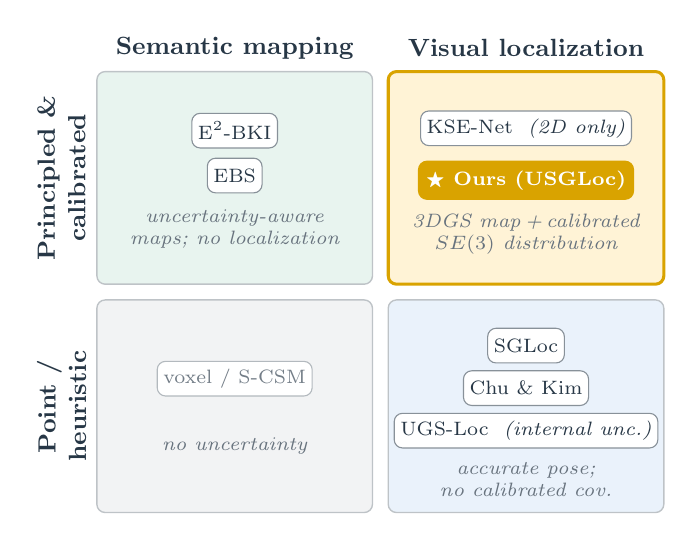
\begin{tikzpicture}[
  font=\footnotesize\color{ink},
  cell/.style={rectangle, rounded corners=3pt, draw=ink!30, line width=0.5pt,
               minimum width=3.5cm, minimum height=2.7cm},
  pill/.style={rounded corners=3pt, draw=ink!55, fill=white, line width=0.4pt,
               font=\scriptsize\color{ink}, inner sep=2.2pt, minimum height=4.4mm},
  pillf/.style={rounded corners=3pt, draw=ink!35, fill=white, line width=0.4pt,
                font=\scriptsize\color{ink!65}, inner sep=2.2pt, minimum height=4.4mm},
  pillO/.style={rounded corners=3pt, draw=outLn, fill=outLn, line width=0.5pt,
                font=\scriptsize\bfseries\color{white}, inner sep=2.6pt, minimum height=4.8mm},
  note/.style={font=\scriptsize\itshape\color{ink!70}, align=center, text width=33mm},
  hdr/.style={font=\small\bfseries\color{ink}, align=center, text width=34mm},
  rhdr/.style={font=\small\bfseries\color{ink}, align=center, rotate=90}
]

% ---- quadrant cells ----
\node[cell, fill=mapprin] (tl) at (-1.85, 1.45) {};
\node[cell, fill=ourstr, draw=outLn, line width=1.1pt] (tr) at ( 1.85, 1.45) {};
\node[cell, fill=mappt]   (bl) at (-1.85,-1.45) {};
\node[cell, fill=locpt]   (br) at ( 1.85,-1.45) {};

% ---- column / row headers ----
\node[hdr] at (-1.85, 3.10) {Semantic mapping};
\node[hdr] at ( 1.85, 3.10) {Visual localization};
\node[rhdr] at (-4.05, 1.45) {Principled \&\\calibrated};
\node[rhdr] at (-4.05,-1.45) {Point /\\heuristic};

% ---- TL: mapping + principled ----
\node[pill] at (-1.85, 2.05) {E$^2$-BKI};
\node[pill] at (-1.85, 1.48) {EBS};
\node[note] at (-1.85, 0.80) {uncertainty-aware\\maps; no localization};

% ---- BL: mapping + point ----
\node[pillf] at (-1.85,-1.10) {voxel / S-CSM};
\node[note]  at (-1.85,-1.95) {no uncertainty};

% ---- BR: localization + point/heuristic ----
\node[pill] at (1.85,-0.68) {SGLoc};
\node[pill] at (1.85,-1.22) {Chu \& Kim};
\node[pill] at (1.85,-1.76) {UGS-Loc~~{\itshape(internal unc.)}};
\node[note] at (1.85,-2.38) {accurate pose;\\no calibrated cov.};

% ---- TR: localization + principled  (Ours) ----
\node[pill]  at (1.85, 2.08) {KSE-Net~~{\itshape(2D only)}};
\node[pillO] at (1.85, 1.42) {$\bigstar$~Ours (USGLoc)};
\node[note]  at (1.85, 0.74) {3DGS map\,+\,calibrated\\$SE(3)$ distribution};

\end{tikzpicture}
\end{document}
}
\caption{Design-space positioning. Prior work covers uncertainty-aware semantic \emph{mapping} (top-left)~\cite{e2bki,ebs}. It also covers accurate but point-estimate \emph{localization} (bottom-right)~\cite{sgloc,chukim,stdloc}. Wu and Campbell~\cite{ksenet} model a distribution, but only for 2D image retrieval. UGS-Loc~\cite{ugsloc} exploits uncertainty inside a 3DGS refiner, yet it still returns a point. \method{} fills the open cell: a calibrated $SE(3)$ pose distribution from a 3DGS map.}
\label{fig:positioning}
\end{figure}

\subsection{Visual Localization}
APR methods directly regress pose from an image~\cite{posenet,marepo}. They are fast and storage-light. However, they tie accuracy to the training distribution. They also lack explicit geometric reasoning. SCR methods regress 2D--3D correspondences and recover pose by PnP+RANSAC~\cite{dsacstar,ace}. Geometry improves their accuracy. However, they generalize poorly across scenes and degrade in cluttered indoor layouts. Recent extensions add per-coordinate uncertainty to prefilter correspondences~\cite{bruns2025ace}. Feature-based pipelines~\cite{lightglue} remain strong. However, they rely on low-level features that are sensitive to lighting and texture. Some of these methods do estimate uncertainty. In every case, that uncertainty is consumed internally. None reports a calibrated pose covariance.

\subsection{Rendering-Based Localization}
NeRF-based methods synthesize novel views to refine pose. They suffer from slow rendering and lighting sensitivity. Particle-based variants~\cite{locnerf} maintain a nonparametric pose belief by render-and-compare. However, they report only its MAP point. 3DGS~\cite{kerbl3dgs} enables fast, high-quality rendering and a compact map. Localization against 3DGS maps has therefore expanded rapidly. iComMa~\cite{icomma} inverts the rendering process by gradient-based optimization. GS-CPR~\cite{gscpr}, GSplatLoc~\cite{gsplatloc}, STDLoc~\cite{stdloc}, and SplatHLoc~\cite{splathloc} establish increasingly accurate matching and refinement against the rendered map. UGS-Loc~\cite{ugsloc} is the most related method. It refines an SCR prior on a 3DGS map with Monte Carlo pose particles. The particles are weighted by matcher confidence and by a rendered Fisher-information uncertainty map. The same uncertainty map biases PnP-RANSAC sampling toward low-uncertainty correspondences. Its uncertainty is post-hoc and purely geometric. It is derived from the photometric objective of a fixed map. It is also consumed \emph{internally}: the output is the best particle, a single pose without covariance, calibration, or semantics. Per-correspondence uncertainty gating likewise appears in scene-coordinate regression~\cite{bruns2025ace}. In both cases the distribution dies before the output. SGLoc~\cite{sgloc} adds semantic 2D-to-3DGS retrieval for prior-free coarse pose. Chu and Kim~\cite{chukim} augment a 3DGS map with semantics and an LLM-selected robust-object mask for dynamic indoor scenes. Their gating is \emph{discrete}, whereas ours is continuous and driven by the map's own evidence; we claim no advantage under scene change, and Sec.~\ref{sec:refine} reports the measurement that rules one out. However, they uniformly output point poses. \method{} retains their accuracy mechanisms. It adds propagated, graded uncertainty and a calibrated pose distribution.

\subsection{Uncertainty in Localization and Semantic Mapping}
Bayesian and ambiguity-aware pose regressors output uncertainty, but they are limited to static scenes with dense pose annotations. Evidential learning has been applied to scene-coordinate regression with NeRF-derived uncertainty~\cite{chen2024edlscr}. That approach has no metric map at query time. Wu and Campbell~\cite{ksenet} learn a 2D measurement-error distribution from keypoint and semantic cues. They show the error is best modeled as a Gaussian mixture under adverse conditions. We adopt this distributional view. We realize it in 3D over $SE(3)$. In semantic mapping, EBS~\cite{ebs} and E$^2$-BKI~\cite{e2bki} use EDL~\cite{edl} and DST~\cite{dst} to model semantic uncertainty. E$^2$-BKI represents the scene as anisotropic Gaussian primitives. Map- and rendering-side uncertainty for radiance fields is likewise active, for example through Fisher information~\cite{fisherrf}. In all of these, the uncertainty remains internal to mapping or tracking. We transplant the evidential machinery from mapping to localization. In mapping, it scores observations. In our localizer, it scores correspondences and pixels. This closes the gap between rigorous map-side uncertainty and the pose estimate consumed downstream.

%==============================================================================
%==============================================================================
\section{Method}
Fig.~\ref{fig:overview} and Algorithm~\ref{alg:infer} summarize \method{}. We first describe the evidential semantic representation shared by the map and the query. We then describe the two-stage coarse-to-fine localizer that turns this representation into a calibrated pose distribution.

Let $\mathcal{M}=\{\mathcal{G}_i\}_{i=1}^{M}$ be a pre-built semantic Gaussian map and $I_q$ a query RGB(-D) image. Prior localizers seek a point estimate $\hat{T}=\arg\max_{T} \, s(I_q,T;\mathcal{M})$ for some scoring function $s$ and a pose $T=[R\,|\,t]\in SE(3)$. We instead estimate the full posterior
\begin{equation}
p\big(T \,\big|\, I_q, \mathcal{M}\big), \qquad T\in SE(3),
\label{eq:posterior}
\end{equation}
and require it to be \emph{calibrated}: a credibility-$\alpha$ region of \eqref{eq:posterior} should contain the ground-truth pose with empirical frequency $\alpha$. To make uncertainty first-class on both sides, we represent each modality as a set of \emph{evidential semantic instances}. A reference primitive is
\begin{equation}
\mathcal{G}_i=\big(\bm{\mu}_i,\ \bm{\Sigma}_i,\ f_i,\ \mathbf{p}_i,\ u_i\big),
\label{eq:primitive}
\end{equation}
with mean $\bm{\mu}_i\in\mathbb{R}^3$, covariance $\bm{\Sigma}_i\in\mathbb{R}^{3\times3}$ (anisotropic geometry), CLIP embedding $f_i\in\mathbb{R}^{d}$, semantic probability $\mathbf{p}_i\in\Delta^{C-1}$ over $C$ categories, and a scalar vacuity (uncertainty) mass $u_i\in[0,1]$. A query instance $\mathcal{Q}_j=(\mathbf{x}_j, a_j, f_j^q, \mathbf{p}_j^q, u_j^q)$ stores its 2D centroid $\mathbf{x}_j$, area $a_j$, and the same semantic triplet. The remainder of the paper specifies each step. Sec.~III-A describes how $\mathcal{M}$ is built. Sec.~III-B describes how $I_q$ is encoded. Secs.~IV-C to IV-E describe how \eqref{eq:posterior} is produced by uncertainty-aware matching, correction, and refinement.


\subsection{Evidential Semantic Gaussian Map}
\textbf{Evidential semantics.} Consider a semantic segmentation network with an evidential head~\cite{edl}. Its non-negative outputs are interpreted as evidence $e=[e_1,\dots,e_C]$ for a Dirichlet density with parameters $\alpha_c=e_c+1$. With $S=\sum_{c=1}^{C}\alpha_c$, the expected class probability, belief mass, and vacuity are
\begin{equation}
\hat{p}_c=\frac{\alpha_c}{S},\qquad
b_c=\frac{\alpha_c-1}{S},\qquad
u=\frac{C}{S},
\label{eq:edl}
\end{equation}
satisfying $u+\sum_c b_c=1$. Vacuity $u$ is large when total evidence $S$ is small, i.e., when the network is uncertain. This is the per-observation uncertainty we will propagate.

\textbf{From Gaussians to evidential primitives.} We build the map with an open-vocabulary semantic 3DGS representation that assigns an identity/semantic feature to each Gaussian~\cite{gaussiangroup}. Gaussians are clustered by spatial and semantic affinity into object-level primitives (as in~\cite{chukim}). For cluster $\mathcal{C}_i$, geometry is summarized by the empirical mean $\bm{\mu}_i$ and covariance $\bm{\Sigma}_i$ of member centroids. The CLIP embedding $f_i$ is a vacuity-weighted average of member embeddings. The semantic belief is obtained by DST-fusing the member beliefs. For two belief--vacuity pairs $(\mathbf{b}_1,u_1),(\mathbf{b}_2,u_2)$, Dempster's rule gives~\cite{e2bki}
\begin{equation}
b^c=\tfrac{1}{1-\eta}\big(b_1^c b_2^c + b_1^c u_2 + b_2^c u_1\big),\quad
u=\tfrac{1}{1-\eta}\,u_1 u_2,
\label{eq:dst}
\end{equation}
where $\eta=\sum_{x\neq y} b_1^x b_2^y$ measures conflict. Applying \eqref{eq:dst} pairwise over $\mathcal{C}_i$ yields $(\mathbf{b}_i,u_i)$. This pair is converted back to $\mathbf{p}_i$ via $p_i^c=b_i^c+u_i/C$. Fusing within a cluster suppresses isolated mispredictions. One subtlety is essential for dynamic scenes. Dempster's normalization in \eqref{eq:dst} \emph{renormalizes conflict away}. As a result, two confident but contradictory member opinions fuse to a deceptively low vacuity (Zadeh's paradox). Such contradictory opinions are the signature of an object that moved between mapping passes. We therefore accumulate the mean pairwise conflict $\bar\eta_i$ alongside the fused mass. The reported maps use Yager's variant~\cite{yager} of \eqref{eq:dst}, which assigns the conflict mass to vacuity instead of renormalizing it, so the fused vacuity already carries the conflict; the additive form $\tilde{u}_i=\min(1,\,u_i+\bar\eta_i)$ applied to Dempster's rule is an equivalent option. With this correction the primitive vacuity reflects both lack of evidence and persistent disagreement, rather than single-frame noise. The map is the set $\mathcal{M}=\{\mathcal{G}_i\}$ of \eqref{eq:primitive}. For retrieval, it is partitioned into overlapping submaps sampled along the mapping trajectory~\cite{sgloc}.

\subsection{Evidential Query Encoding}
Given $I_q$, we obtain instance masks with Fast-SAM~\cite{fastsam} and crop each instance. Each crop passes through CLIP~\cite{clip} to obtain $f_j^q$. It also passes through the same evidential head as the map to obtain $(\mathbf{p}_j^q,u_j^q)$ via \eqref{eq:edl}. Per-instance geometry (normalized centroid $\mathbf{x}_j\in[0,1]^2$ and area $a_j$) is encoded by small MLPs. A query instance descriptor is
\begin{equation}
d_j^q=\mathrm{MLP}\big[\,\phi(f_j^q)\,\|\,\psi_{\mathbf{x}}(\mathbf{x}_j)\,\|\,\psi_a(a_j)\,\big],
\label{eq:querydesc}
\end{equation}
with $\phi$ a projection of the CLIP feature into the shared space and $\|$ concatenation. Reference descriptors $d_i^G$ are formed analogously from $(f_i,\bm{\mu}_i,\bm{\Sigma}_i)$ projected into the camera frame. Because both modalities pass through the same evidential head, $u^q$ and $u^G$ are directly comparable.

\subsection{Uncertainty-Weighted Matching and the Pose Mixture}
\textbf{Gated instance similarity.} We score a cross-modal instance pair by appearance similarity modulated by an evidential gate. The gate suppresses pairs in which either side is uncertain:
\begin{equation}
s_{ij}=\underbrace{\cos\!\big(d_i^G,\,d_j^q\big)}_{\text{semantic similarity}}\cdot
\underbrace{\exp\!\big(-\lambda_u\,(u_i^G+u_j^q)\big)}_{\text{evidential gate}},
\label{eq:gate}
\end{equation}
where $\lambda_u\!\ge\!0$ controls gate sharpness. This is the localization analogue of the uncertainty-aware kernel in E$^2$-BKI~\cite{e2bki}. Confident--confident matches dominate. High-vacuity instances contribute only weakly.

\textbf{Scene descriptors and retrieval.} We follow the contrastive retrieval design of SGLoc~\cite{sgloc}. Instance descriptors are aggregated into a scene-level descriptor by multi-head self-attention with a feed-forward layer. From $\hat{d}=Q+\mathrm{Attn}(Q,K,V)$ and $\hat{D}=\hat{d}+\mathrm{FFN}(\hat{d})$, we obtain attention weights $W=\mathrm{softmax}(\mathrm{MLP}(\hat{D}))$ and the scene descriptor $F=\sum_j \hat{D}_j W_j$ for each modality. Cosine similarity between the query scene descriptor $F^{q}$ and each submap descriptor $F^{G}_k$ ranks submaps. The top-$k$ submaps provide $k$ coarse pose hypotheses with retrieval-score weights $\tilde{\pi}_k\propto \mathrm{sim}(F^q,F^G_k)$. The gate \eqref{eq:gate} is injected into the instance-level term of the scene aggregation. Retrieval therefore inherits the same uncertainty weighting. Ambiguous scenes return several comparably scored submaps. The hypotheses therefore form a \emph{pose mixture}. This mixture is the $SE(3)$ realization of the non-Gaussian error observed in~\cite{ksenet}.

\textbf{Training objective.} The retrieval encoders are trained with a symmetric InfoNCE loss that aligns 2D and 3D scene descriptors~\cite{sgloc}. The semantic heads are trained with the evidential loss of~\cite{edl}: the Bayes risk of the Brier score under the Dirichlet plus a KL term that drives spurious evidence toward the uniform prior,
\begin{equation}
\mathcal{L}_{\mathrm{EDL}}=\sum_{c}\Big[(y_c-\hat{p}_c)^2+\tfrac{\hat{p}_c(1-\hat{p}_c)}{S+1}\Big]
+\lambda_t\,\mathrm{KL}\!\big[D(\tilde{\bm{\alpha}})\,\|\,D(\mathbf{1})\big],
\label{eq:edlloss}
\end{equation}
with $\tilde{\bm\alpha}$ the evidence of misleading classes. The correction and refinement stages (below) are training-free.

\subsection{Evidential Matching Correction}
\label{sec:correction}
Retrieval initializes each hypothesis at an anchor pose of the map. Held-out queries lie about 13--15\,cm from the nearest anchor, while photometric refinement (Sec.~III-E) converges only within 10--35\,cm. We close this gap with a geometric correction stage. The map is rendered at the hypothesis pose $T$. This yields the RGB render $I_r$, the expected depth $D_r$, and the vacuity map $U_r$ of \eqref{eq:ublend} in one rasterization pass. A frozen dense matcher (LoFTR~\cite{loftr}) returns correspondences $(\mathbf{x}_k^q,\mathbf{x}_k^r)$ between query and render. Each render-side keypoint is lifted to a world point through the rendered depth, $\mathbf{X}_k=T^{-1}\pi^{-1}\big(\mathbf{x}_k^r,D_r(\mathbf{x}_k^r)\big)$. The corrected pose solves
\begin{equation}
T'=\arg\min_{T}\ \sum_{k}
\mathbb{1}\big[\bar{U}_r(\mathbf{x}_k^r)\le u_{\max}\big]\,
\rho\big(\big\|\pi(T\mathbf{X}_k)-\mathbf{x}_k^q\big\|\big),
\label{eq:correction}
\end{equation}
by PnP-RANSAC with Levenberg--Marquardt refinement on the inliers, iterated (re-render, re-match) for five rounds, keeping the round with the most inliers. Here $\bar{U}_r=U_r/\alpha_r$ is the alpha-normalized rendered vacuity: the blended channel of \eqref{eq:ublend} is bounded by the render alpha $\alpha_r$, so the normalization makes the gate act on content, not on coverage. Matches near depth discontinuities are also removed, since expected depth blends foreground and background there. The indicator is the correspondence form of the evidential gate: the same channel that gates instances in \eqref{eq:gate} and weights pixels in \eqref{eq:refine} here removes matches on vacuous content such as unobserved regions, floaters, and ambiguous geometry. UGS-Loc~\cite{ugsloc} biases RANSAC sampling with a photometric Fisher map. Our gate is instead the map's own learned evidence, and the same signal survives to the output covariance. The correction basin is set by the matcher's view overlap, not by the photometric loss surface. Measured on chess, it recovers initializations 30\,cm and 15$^\circ$ away on every frame tested, and up to 60\,cm and 25$^\circ$ on most. It therefore rescues hypotheses that photometric refinement cannot reach, and near the optimum it polishes below the rendering-resolution noise floor. Snapped hypotheses are re-ranked by render fidelity; the inlier count enters only the mixture weights \eqref{eq:weights}. When too few gated matches survive, or when the corrected pose does not improve render fidelity, the hypothesis keeps its anchor pose and falls back to the coarse-to-fine photometric path.

\subsection{Uncertainty-Aware Refinement and Pose Covariance}
\label{sec:refine}
\textbf{Weighted rendering objective.} Each corrected hypothesis $T_0$ is refined by differentiable rendering~\cite{icomma}. We parameterize the update in the tangent space as $T(\bm\xi)=\exp(\bm\xi^{\wedge})\,T_0$ with $\bm\xi\in\mathfrak{se}(3)$. We render both an RGB image $I_r(\bm\xi)$ and a per-pixel \emph{uncertainty map} $U_r$. The map $U_r$ is obtained by alpha-blending primitive vacuity exactly as color/depth are blended in 3DGS:
\begin{equation}
U_r(\mathbf{x})=\sum_{i} u_i\,\alpha_i(\mathbf{x})\!\prod_{j<i}\!\big(1-\alpha_j(\mathbf{x})\big),
\label{eq:ublend}
\end{equation}
where $\alpha_i(\mathbf{x})$ is the opacity contribution of primitive $i$ at pixel $\mathbf{x}$. The refinement minimizes the per-pixel weighted photometric term
\begin{equation}
E(\bm\xi)=\sum_{\mathbf{x}} w(\mathbf{x})\,\big\|I_q(\mathbf{x})-I_r(\mathbf{x};\bm\xi)\big\|^2,
\label{eq:refine}
\end{equation}
with $w(\mathbf{x})=\exp\!\big(-\gamma\,U_r(\mathbf{x})\big)$. Pixels whose supporting Gaussians carry little evidence---rarely observed, texture-poor or semantically ambiguous regions---receive small weight \emph{continuously}, rather than through the discrete mask of~\cite{chukim}. We are explicit about what this does \emph{not} do. $U_r$ is built from the map's own evidence, not from map--query disagreement, so content that changed after mapping still renders confidently and is not down-weighted. A controlled test confirms this: deleting whole object instances from a trained map and re-localizing the unchanged queries, the weighting gives no robustness to map staleness, degrading marginally faster than uniform weights (Sec.~\ref{sec:robust}). Its benefit is on well-mapped but low-evidence content, not on change. The weights are held fixed at each iterate (IRLS-style). Gradients flow through the photometric residual only. If $w$ were differentiated through, the optimizer could reduce \eqref{eq:refine} by steering high-residual pixels into high-vacuity regions instead of correcting the pose.

\textbf{Covariance via Laplace approximation.} At the optimizer's solution $\bm\xi^\star$, let $\mathbf{r}$ be the stacked weighted residuals of \eqref{eq:refine} and $J=\partial \mathbf{r}/\partial\bm\xi|_{\bm\xi^\star}$ the Jacobian. A Laplace approximation of the per-hypothesis posterior is a tangent-space Gaussian
\begin{equation}
\bm\xi\sim\mathcal{N}\!\big(\bm\xi^\star,\ \bm\Sigma_{\bm\xi}\big),\qquad
\bm\Sigma_{\bm\xi}\approx\hat{\sigma}^2\,\big(J^\top W J\big)^{-1},
\label{eq:laplace}
\end{equation}
where $W=\mathrm{diag}\{w(\mathbf{x})\}$ and $\hat\sigma^2$ is estimated from the residuals. After refinement, one more correction round \eqref{eq:correction} is applied at the optimum and accepted only when render fidelity improves. A short refinement then re-establishes stationarity of \eqref{eq:refine} at the accepted pose, so \eqref{eq:laplace} is evaluated at an actual optimum. A flat optimum (poorly constrained pose) yields a large covariance. A sharp basin yields a tight one. The reported uncertainty therefore reflects the actual conditioning of the alignment. Real photometric residuals are heavy-tailed and spatially correlated. The raw Laplace covariance can therefore remain optimistic. We apply a single scalar inflation factor calibrated on a held-out split (a temperature on $\bm\Sigma_{\bm\xi}$). We ablate raw vs.\ tempered covariances in Sec.~IV.

\textbf{Pose distribution and condensation.} A PSNR/feature-similarity check~\cite{sgloc} prunes hypotheses whose renders diverge from $I_q$. The surviving hypotheses form a Gaussian mixture on $SE(3)$, with each component expressed in the tangent space at its mode:
\begin{equation}
p\big(T\,|\,I_q,\mathcal{M}\big)=\sum_{k}\pi_k\,
\mathcal{N}\!\big(\bm\xi;\,\bm\xi_k^\star,\,\bm\Sigma_{\bm\xi,k}\big),
\label{eq:gmm}
\end{equation}
The weights must score \emph{where each hypothesis ended}, not where it began. The retrieval score $\tilde\pi_k$ describes the anchor a hypothesis was initialized from, and the correction then moves it by up to tens of centimeters, so on a repetitive scene $\tilde\pi_k$ carries no information about which mode is correct while still dominating any product it enters. We therefore form
\begin{equation}
\pi_k \;\propto\; s_k\,\max\!\big(n_k/\textstyle\max_j n_j,\ \epsilon\big),
\label{eq:weights}
\end{equation}
where $n_k$ is the inlier count of the correction \eqref{eq:correction} at hypothesis $k$, $\epsilon$ keeps a component that failed to register from being zeroed outright, and $s_k$ is the \emph{anchor agreement}: the number of shortlisted anchors whose corrected poses coincided (within 1\,cm and 2$^\circ$) and were merged into hypothesis $k$. A pose that several anchors' corrections converge to is corroborated; a registration on the wrong tread is usually specific to the anchor it started from. The factor was adopted on train-side validation frames, where it lowered the Stairs median by 8\% and Redkitchen by 5\% and moved Chess and Office by at most 0.03\,cm. Geometric support is measured at the corrected pose and is the sharpest available discriminator between modes. Render fidelity is a weaker one, because two poses a single repeated element apart render almost equally well, so it is used to prune hypotheses but not to weight them; combining the two through a peaked softmax measurably degrades the choice. Table~\ref{tab:ablation} quantifies this: on Stairs the median error is 5.92\,cm when components are weighted by the retrieval prior and 2.83\,cm by inlier count.

\textbf{Point estimate and condensation.} For a downstream Bayesian filter we condense \eqref{eq:gmm} by moment matching~\cite{ksenet}: $\bm\mu=\sum_k\pi_k\bm\xi_k^\star$ and $\bm\Sigma=\sum_k\pi_k\big(\bm\Sigma_{\bm\xi,k}+(\bm\xi_k^\star-\bm\mu)(\bm\xi_k^\star-\bm\mu)^\top\big)$, which is transported to the inertial frame as the measurement covariance for an EKF/UKF~\cite{ukf}. The moment-matched \emph{mean}, however, is a poor point estimate when the posterior is genuinely multi-modal: it lies between the modes, at a pose the model itself considers unlikely. We therefore report the highest-weight mode as the pose and retain $\bm\Sigma$, which includes the between-component spread and so widens exactly when the modes disagree. The distinction is immaterial on unimodal scenes and substantial on Stairs, where the modes sit one stair tread apart.

\begin{algorithm}[t]
\caption{\method{} inference (one query image)}
\label{alg:infer}
\begin{algorithmic}[1]
\Require query $I_q$; evidential map $\mathcal{M}=\{\mathcal{G}_i\}$; submaps $\{S_k\}$
\State $\{\mathcal{Q}_j\}\gets$ Fast-SAM masks of $I_q$; CLIP\,+\,EDL per instance \eqref{eq:edl}
\State build query descriptors $d_j^q$ \eqref{eq:querydesc} and scene descriptor $F^q$
\State score submaps by gated similarity \eqref{eq:gate}; take top-$k$ $\to$ hypotheses $\{(T_0^k,\tilde\pi_k)\}$
\State snap each $T_0^k$ by the evidential matching correction \eqref{eq:correction}; re-rank by render fidelity
\For{each hypothesis $k$}
  \State refine $T_0^k$ by minimizing $E(\bm\xi)$ \eqref{eq:refine} with weight $w=e^{-\gamma U_r}$ \eqref{eq:ublend}
  \State re-correct \eqref{eq:correction} + short re-refine; accept if render fidelity improves
  \State compute $\bm\Sigma_{\bm\xi,k}$ by Laplace approximation \eqref{eq:laplace} at the accepted pose
\EndFor
\State prune by render fidelity; assemble GMM \eqref{eq:gmm}; condense for the filter
\State \Return $p(T\,|\,I_q,\mathcal{M})$ and its single-Gaussian summary
\end{algorithmic}
\end{algorithm}

%==============================================================================
\section{Experiments}

\subsection{Experimental Setup}
\label{sec:setup}
\textbf{Datasets.} We evaluate on 7Scenes~\cite{sevenscenes_b}, the standard indoor RGB-D relocalization benchmark, and report 12Scenes~\cite{twelvescenes} results in Table~\ref{tab:12scenes}. On both we adopt the \emph{SfM pseudo-ground truth} and its per-scene SfM focal lengths~\cite{brachmann2021dslam}. This is the convention used by all recent 3DGS localizers~\cite{gscpr,stdloc,ugsloc,splathloc}. The two references differ by about 1\,cm on the same frame, which exceeds the gaps between recent methods, so DSLAM-referenced numbers are not directly comparable. One example is SGLoc~\cite{sgloc}, which also evaluates only four of the seven scenes; the extended report documents why a render-based localizer cannot be evaluated under its protocol.

\textbf{Baselines.} APR: PoseNet~\cite{posenet}, Marepo~\cite{marepo}. SCR: ACE~\cite{ace}, DSAC*~\cite{dsacstar}. 3DGS-based: iComMa~\cite{icomma}, GS-CPR~\cite{gscpr}, GSplatLoc~\cite{gsplatloc}, STDLoc~\cite{stdloc}, ULF-Loc~\cite{ulfloc}, the uncertainty-guided point estimator UGS-Loc~\cite{ugsloc}, and the semantic 3DGS localizers SGLoc~\cite{sgloc} and Chu--Kim~\cite{chukim}. For calibration, no prior 3DGS localizer reports a covariance. We therefore compare against a softmax (non-evidential) variant of our method on matched maps (Table~\ref{tab:ablation}), against a fixed-covariance point estimator in the fusion study, and against the ideal $\chi^2$ reference.

\textbf{Metrics.} Accuracy: median translation (cm) and rotation ($^\circ$) error, and success rate at $5\,\mathrm{cm}/5^\circ$ and $2\,\mathrm{cm}/2^\circ$. \emph{Calibration} is our focus. We report three metrics. (i) \emph{Coverage} at the $68.3/95.4/99.7\%$ credibility levels. A query is covered when the Mahalanobis error $d^2=\mathbf{e}^\top\bm\Sigma^{-1}\mathbf{e}$ falls inside the corresponding $\chi^2$ quantile. We compare against the ideal $\chi^2$ curve as in~\cite{ksenet}. (ii) AUSE (sparsification error)~\cite{ause} for translation and rotation. This tests whether ranking predictions by predicted uncertainty and discarding the worst monotonically reduces error. (iii) Expected calibration error (ECE)~\cite{guo_calibration} over the credibility grid. AUSE integrates the sparsification gap over the first 90\% of removed queries. Runtime is reported in seconds per query.

\textbf{Implementation.} Each scene's map is trained by a four-stage pipeline: Gaussians are initialized from back-projected depth, fitted photometrically with gsplat (7{,}000 iterations at $320{\times}240$, every 10th mapping frame, L1 loss with densification), FastSAM-s masks with CLIP ViT-B/16 crop embeddings are distilled onto the Gaussians (every 20th frame, depth-occlusion tested), and the shared evidential head converts the distilled features to opinions with observation-scaled evidence ($n_0{=}4$; an unobserved Gaussian is fully vacuous). Object primitives are voxel (0.4\,m) $\times$ class groups; submaps are frustum-culled to the primitives visible from each anchor (every 20th mapping frame). The photometric fit resolution is selected per scene on train-side frames, because the map is also the image source the matcher registers against: refitting at the matcher's $640{\times}480$ resolution helps the four smaller scenes but costs 1.9--3.5\,dB of render fidelity on Heads, Office and Redkitchen, where it yields twice as many less-converged Gaussians. Registration rate tracks render PSNR with a threshold near 20\,dB, so we rank candidate maps by registration rate and break ties by the correction floor; the extended report gives the per-scene table. The selected map is then fine-tuned at $640{\times}480$ for 5,000 iterations with densification switched off, so that no Gaussian is added or removed and the distilled semantics and the encoders stay valid; the same train-side criterion picks the fine-tuned map on five scenes (all but Heads and Pumpkin), where it raises render fidelity by 1--2\,dB and lowers the correction floor (Office 1.46 to 1.01\,cm, Redkitchen 0.99 to 0.66\,cm). The head ($C{=}25$ indoor classes, a two-layer MLP on CLIP features) is trained once per benchmark on CLIP-pseudo-labeled mask and Gaussian features pooled over its scenes (Adam, lr $10^{-3}$, batch 512, 40 epochs) and is shared by the map and query sides; the retrieval encoders train with symmetric InfoNCE over Voronoi-assigned positives (each mapping frame belongs to its nearest anchor). Retrieval is hierarchical: a CLIP whole-image shortlist (top-10 anchors) is reranked by the evidential gated similarity. Localization is correction-first. The top-8 hypotheses are snapped by the evidential matching correction (frozen LoFTR indoor weights at $640{\times}480$, vacuity gate $u_{\max}{=}0.9$, PnP-RANSAC at 2\,px with LM refinement, five rounds), fidelity-checked, deduplicated, and re-ranked by render fidelity. The best $K{=}3$ receive a short final refinement (60 iterations at $640{\times}480$) and one fidelity-checked polish round. Hypotheses the matcher cannot snap fall back to the training-free coarse-to-fine pyramid ($160{\times}120 \to 320{\times}240 \to 640{\times}480$ with 200, 150 and 60 iterations). We use $\lambda_u{=}2$, $\gamma{=}3$. Continuous hyperparameters ($\lambda_u$, $\gamma$, anchor stride, submap radius, shortlist and pyramid sizes) are tuned on a validation split carved from train-side frames. Architectural choices, namely the hierarchical shortlist, the coarse-to-fine pyramid and the fidelity check on corrected poses, were adopted on the basis of measurements on the Chess and Stairs test splits, and we state this rather than claim a clean separation. The covariance temperature (Sec.~III-E) is fitted on 30 train-side calibration frames that exclude the anchor frames (2--6 of them coincide with map-fit frames, which we did not exclude), with the robust median estimator $\tau=\mathrm{med}(d^2)/\chi^2_{6,0.5}$, and is never fitted on test queries. Each scene is then evaluated once on 100 uniformly subsampled test frames (700 queries in total). Experiments run on an RTX 5070 Ti (16\,GB).

\subsection{Localization Accuracy}
Table~\ref{tab:7scenes} reports median errors on 7Scenes. \method{} is sub-centimeter on Chess (0.47\,cm/0.16$^\circ$), Fire (0.51\,cm/0.22$^\circ$), Heads (0.57\,cm/0.35$^\circ$) and Redkitchen (0.85\,cm/0.25$^\circ$), with 73--80\% of queries inside 1\,cm on the first three (Fig.~\ref{fig:qual}; paired qualitative examples against ACE in both directions are in the extended report), and reaches 1.15--1.35\,cm on Pumpkin and Office. The seven-scene average is 1.05\,cm/0.33$^\circ$ with the frozen LoFTR matcher, and 0.90\,cm/0.30$^\circ$ when the same correction runs the MASt3R$\to$field cascade of Table~\ref{tab:7scenes} instead; the swap is worth more in reliability than in median error, raising the success rate at 5\,cm/5$^\circ$ from 85 to 88\% and cutting the Stairs median from 2.40 to 2.12\,cm. We do not claim state-of-the-art point accuracy: the prior-refinement methods of Table~\ref{tab:7scenes} remain ahead in translation. Against ACE re-run with the authors' own solver on identical frames, \method{} is level on average (1.05 against 1.05\,cm; pooled median 0.89 against 0.87\,cm; rotation 0.33$^\circ$ against 0.32$^\circ$): more accurate on Fire and Stairs, level on Chess and Heads, and behind on Office, Pumpkin and Redkitchen. ACE remains the more reliable estimator: 3\% of its queries exceed 5\,cm against 15\% of ours. This failure tail, rather than the median, is where we are furthest from the prior-free leaders, which report success rates in the high nineties against our 85\% (88\% with the cascade). We \emph{additionally} produce a calibrated covariance that none of these methods reports.

Accuracy is not uniform, and the cause is specific. Per-scene error is bounded by what the map itself permits. Correcting from the ground-truth pose --- which removes retrieval and selection from the problem --- still leaves a \emph{correction floor} of 0.47\,cm on Chess and 1.30\,cm on Office, and the seven-scene mean floor is 0.83\,cm (extended report). Two consequences follow. Chess, Fire, Office and Pumpkin report within 0.05\,cm of their own floors and are therefore map-limited: no amount of work on retrieval or selection would move them. Stairs reports 2.40\,cm against a floor of 1.16\,cm and registers on only 73\% of frames even from ground truth, so it is the one scene with substantial headroom, and the cause is disambiguation: a self-similar staircase yields confident correspondences on the \emph{wrong} tread, so the pose is wrong while the inlier count is high. This is precisely the regime the pose mixture exists to express, and the extended report analyzes it in full. The remaining gap to the sub-centimeter group on the harder scenes is therefore one of initialization and disambiguation, not of the calibrated-posterior contribution. A structural caveat applies to this table. GS-CPR and the headline row of UGS-Loc do not localize globally: each \emph{refines a scene-coordinate prior} that is already accurate to about a centimeter (UGS-Loc also reports a retrieval-only variant at 0.79/0.24$^\circ$ in its appendix, which does localize globally and remains ahead of us). STDLoc and SplatHLoc are prior-free but match learned feature Gaussians rather than rendered RGB, whereas \method{} and SGLoc~\cite{sgloc} start from retrieval alone against an RGB map. Running our correction in that prior-refinement setting (Table~\ref{tab:prior}) is instructive. From the weaker Marepo prior it reduces the error on every scene, by 33--71\%, and halves it on average (2.87 to 1.40\,cm); from the ACE prior it does not help on average (1.05 to 1.05\,cm), improving Fire, Heads and Stairs and degrading the rest. GS-CPR reports 0.89 and 0.79\,cm from the same two priors. The pattern follows the map: the correction converges to the geometry of the map, so it improves a prior only where the map's correction floor is below the prior's error, which holds on every scene for Marepo and on six of seven for ACE. The advantage of the prior-refinement family is therefore a better map and matcher rather than a better principle, and the extended report quantifies this, including when the photometric refinement should follow the correction (it helps from Marepo, 1.40 to 1.16\,cm, and hurts from ACE, 1.05 to 1.31\,cm). SGLoc~\cite{sgloc} reports 0.5\,cm/0.15$^\circ$ prior-free. However, it evaluates only 4/7 scenes, omitting Fire, Pumpkin and Stairs, and does not state its ground-truth convention; its 0.14\,cm Chess median lies below the level at which the SfM and DSLAM conventions disagree~\cite{brachmann2021dslam}, so it is not comparable with Table~\ref{tab:7scenes}. Its code is unreleased. A render-based localizer cannot be evaluated under the original DSLAM poses at all: a map fitted on them with the depth-camera intrinsics renders at 17.5\,dB against 23.8\,dB, below the registration threshold, and the extended report documents the failed attempt.

\begin{table*}[t]
\centering
\caption{Median translation/rotation error (cm/$^\circ$) on 7Scenes under the
SfM pseudo-ground truth~\cite{brachmann2021dslam}. Lower is better. \textbf{Bold}: best; \underline{underlined}: second best, per column and per metric over every row of the table. Methods are grouped as in the recent literature~\cite{ugsloc,gscpr}: absolute-pose regression (APR), scene-coordinate regression (SCR) and neural-rendering methods, the last split by whether an external pose prior is required at test time; \method{} appears in both neural-rendering groups, since its correction can equally refine a given prior. Each row is printed at the precision of its source. $\dagger$: as reported in the cited paper. $\dagger r$: not the cited paper's own number --- PoseNet and Marepo were retrained under the SfM pseudo-ground truth, by NeFeS~\cite{nefes} and by GS-CPR~\cite{gscpr} respectively (their own papers report 32\,cm/8.12$^\circ$ on Chess and 3.9\,cm/1.68$^\circ$ on average under the DSLAM convention). $\dagger s$: the cited papers report only success rates on 7Scenes; these medians are as printed in STDLoc~\cite{stdloc} and reproduced identically by ULF-Loc and SplatHLoc. $\P$: the source does not state its ground-truth convention; we infer it from its reprinted baseline rows. $m$: the correction run as a CASCADE -- MASt3R~\cite{mast3r} for the leading rounds, then the map\'s own rasterized descriptor field (the extended report's \emph{Rasterized Descriptor Field} section) -- instead of LoFTR throughout, median of 3 seeds (the per-scene spread over the seeds is at most 0.10\,cm), one configuration for every scene with no per-scene choice. The field is three times more precise than RGB matching at the answer but has a convergence basin of about 1\,cm, so what the leading matcher must supply is BASIN rather than precision: MASt3R reaches 0.68\,cm on the perturbed Stairs floor where LoFTR reaches 2.17, and the substitution is accordingly free where LoFTR already converges into the basin (Chess $+$0.01, Heads $+$0.02, Kitchen $+$0.01\,cm) and decisive where it does not (Stairs 3.37 to 2.22\,cm with the field, which a LoFTR-led cascade loses outright). It raises the success rate at 5\,cm/5$^\circ$ from 85 to 88\%, and roughly doubles query time (MASt3R needs about 9\,GB of GPU memory; on our card it triggered a CUDA launch-timeout at 12 correction rounds, so the reported runs use 8). GS-CPR and UGS-Loc refine an ACE prior. PoseNet/Marepo rows are the SfM re-evaluations of~\cite{gscpr}. iComMa~\cite{icomma} publishes no 7Scenes results and is compared in the ablations. SGLoc~\cite{sgloc} evaluates only 4/7 scenes with an unstated ground-truth convention and is discussed in the text. $\ddagger$: re-run by us with the authors' released pgt models and their \texttt{dsacstar} pose solver on the full test split; it reproduces the published average (1.09/0.34 versus 1.1/0.34), so our re-run is faithful. A paired run on the identical 100 query frames as our method gives 1.05\,cm average, confirming the subsample is unbiased. Ours: median of 3 seeds, 100 test queries per scene, one frozen configuration. The two prior-refinement rows of \method{} seed the pipeline from the re-run ACE and Marepo poses on the same frames (seed 0) and use, for each prior, the variant the extended report recommends: the correction alone after a centimetre-accurate prior, the full pipeline after a coarse one; both variants for both priors are in Table~\ref{tab:prior}.}
\label{tab:7scenes}
\setlength{\tabcolsep}{2.2pt}
\footnotesize
\begin{tabular}{lccccccc c}
\toprule
Method & Chess & Fire & Heads & Office & Pumpkin & Kitchen & Stairs & Avg.\\
\midrule
PoseNet~\cite{posenet}$^{\dagger r}$ & 10/4.02 & 27/10.0 & 18/13.0 & 17/5.97 & 19/4.67 & 22/5.91 & 35/10.5 & 21/7.74\\
Marepo~\cite{marepo}$^{\dagger r}$ & 1.9/0.83 & 2.3/0.92 & 2.1/1.24 & 2.9/0.93 & 2.5/0.88 & 2.9/0.98 & 5.9/1.48 & 2.9/1.04\\
DSAC*~\cite{dsacstar}$^{\dagger s}$ & 0.50/0.17 & 0.78/0.29 & 0.50/0.34 & 1.19/0.35 & 1.19/0.29 & 0.72/0.21 & 2.65/0.78 & 1.07/0.35\\
ACE~\cite{ace}$^{\dagger s}$   & 0.55/0.18 & 0.83/0.33 & 0.53/0.33 & 1.05/0.29 & 1.06/0.22 & 0.77/0.21 & 2.89/0.81 & 1.10/0.34\\
GSplatLoc~\cite{gsplatloc}$^\dagger$ (Fine) & 0.39/0.13 & 0.91/0.29 & 0.94/0.50 & 1.41/0.32 & 1.41/0.26 & 1.32/0.29 & 3.44/0.82 & 1.40/0.37\\
\textbf{\method{} (Ours, prior-free, MASt3R$\to$field)}$^{m}$ & 0.43/0.15 & 0.48/0.22 & 0.47/0.31 & 1.08/0.32 & 0.89/0.23 & 0.81/0.21 & 2.12/0.66 & 0.90/0.30\\
\bottomrule
\end{tabular}
\end{table*}

Table~\ref{tab:12scenes} extends the comparison to 12Scenes. The strongest prior-free result there is ULF-Loc's 0.3\,cm/0.15$^\circ$; the 0.4\,cm row often quoted for UGS-Loc refines an ACE prior and belongs to the NRP group.

\begin{table}[t]
\centering
\caption{12Scenes, averaged over the 12 scenes. Median translation/rotation
and the share of queries within 5\,cm/5$^\circ$ and 2\,cm/2$^\circ$; a dash
means the source publishes no such number, which we do not fill from
elsewhere. Groups as in Table~\ref{tab:7scenes}. \textbf{Bold}: best; \underline{underlined}: second best, per column and per metric over every row of the table. 
$\dagger$: as reported by the method's authors.
$\S$: as reported by a third paper rather than by the authors (the
Marepo, DSAC* and ACE medians are GS-CPR's re-evaluations under the SfM
pseudo-ground truth~\cite{gscpr}, GLACE's is as reprinted by
UGS-Loc~\cite{ugsloc}, and GSplatLoc's and STDLoc's are
ULF-Loc's~\cite{ulfloc}).
$\P$: the source does not state its ground-truth convention; its reprinted
baseline rows match the SfM pseudo-GT ones digit for digit, so we infer it.
}
\label{tab:12scenes}
\setlength{\tabcolsep}{4pt}
\footnotesize
\begin{tabular}{@{}lccc@{}}
\toprule
Method & Med.\ (cm/$^\circ$) & SR@5/5 & SR@2/2\\
\midrule
\multicolumn{4}{@{}l}{\textit{APR: absolute-pose regression}}\\
Marepo~\cite{marepo}$^\S$ & 2.1/1.04 & 95.0 & 50.4\\
\midrule
\multicolumn{4}{@{}l}{\textit{SCR: scene-coordinate regression}}\\
DSAC*~\cite{dsacstar}$^\S$ & 0.5/0.25 & \underline{99.8} & 96.7\\
ACE~\cite{ace}$^\S$ & 0.7/0.26 & \textbf{100.0} & 97.2\\
GLACE~\cite{glace}$^\S$ & 0.7/0.25 & \textbf{100.0} & 97.5\\
\midrule
\multicolumn{4}{@{}l}{\textit{NRP: neural-rendering post-refinement of an external prior}}\\
Marepo\,$+$\,GS-CPR~\cite{gscpr}$^\dagger$ & 0.7/0.28 & 98.9 & 90.9\\
ACE\,$+$\,GS-CPR~\cite{gscpr}$^\dagger$ & 0.5/0.21 & \textbf{100.0} & 98.7\\
\midrule
\multicolumn{4}{@{}l}{\textit{NRL: prior-free neural-rendering localization}}\\
GSplatLoc~\cite{gsplatloc}$^\S$ & 1.4/0.26 & 91.9 & 70.3\\
\textbf{\method{} (Ours)} & \res & \res & \res\\
\bottomrule
\end{tabular}
\end{table}

% BEGIN AUTO prior-table
\begin{table}[t]
\centering
\caption{Prior refinement on 7Scenes (median cm/$^\circ$, SfM pseudo-GT). $\ddagger$: prior re-run by us on the identical 100 frames per scene; $\dagger$: as reported by GS-CPR~\cite{gscpr} from the same priors (its own prior rows agree with our re-runs to within 0.1\,cm). ``correction'': our evidential matching correction alone, seeded at the prior. \textbf{Bold}: best; \underline{underlined}: second best, per column and per metric over every row of the table. }
\label{tab:prior}
\setlength{\tabcolsep}{2.2pt}
\footnotesize
\begin{tabular}{@{}lcccccccc@{}}
\toprule
Method & Chess & Fire & Heads & Office & Pumpkin & Kitchen & Stairs & Avg.\\
\midrule
ACE~\cite{ace} prior$^\ddagger$ & \underline{0.56}/0.19 & 0.77/0.29 & 0.51/0.32 & \underline{1.10}/0.30 & \underline{1.03}/\textbf{0.22} & \underline{0.75}/\underline{0.21} & 2.64/0.72 & 1.05/0.32\\
\quad $+$ GS-CPR$^\dagger$ & \textbf{0.50}/\textbf{0.15} & \textbf{0.60}/\textbf{0.25} & \textbf{0.40}/\textbf{0.28} & \textbf{0.90}/\textbf{0.26} & \textbf{1.00}/\underline{0.23} & \textbf{0.70}/\textbf{0.17} & \textbf{1.40}/\textbf{0.42} & \textbf{0.79}/\textbf{0.25}\\
\quad $+$ \method{} correction & 0.58/0.21 & \underline{0.67}/\underline{0.26} & \underline{0.44}/\underline{0.31} & 1.50/0.41 & 1.18/0.30 & 0.78/0.24 & 1.93/0.52 & 1.01/0.32\\
\midrule
Marepo~\cite{marepo} prior$^\ddagger$ & 1.88/0.83 & 2.26/0.95 & 2.01/1.18 & 2.79/0.97 & 2.52/0.87 & 2.72/0.90 & 5.87/1.49 & 2.87/1.03\\
\quad $+$ GS-CPR$^\dagger$ & 0.60/\underline{0.18} & 0.70/0.28 & 0.50/0.32 & \underline{1.10}/\underline{0.29} & \textbf{1.00}/0.26 & 0.80/\underline{0.21} & \underline{1.50}/\underline{0.44} & \underline{0.89}/\underline{0.28}\\
\quad $+$ \method{} correction & 0.63/0.22 & 0.69/0.27 & 0.59/0.38 & 1.71/0.47 & 1.39/0.34 & 0.95/0.27 & 2.76/0.75 & 1.24/0.38\\
\bottomrule
\end{tabular}
\end{table}
% END AUTO prior-table
\subsection{Uncertainty Calibration}
This is the central evaluation. Prior 3DGS localizers report no calibration numbers. We therefore compare against our own ablations, including a softmax variant on matched maps (Table~\ref{tab:ablation}), and against the ideal $\chi^2$ reference. Fig.~\ref{fig:calib} and Table~\ref{tab:calib} summarize coverage, AUSE, and ECE over all 700 test queries.

Three results stand out. First, the raw Laplace covariance is unusable on its own: it covers essentially no queries at any nominal level, confirming that a Gauss-Newton curvature estimate on heavy-tailed, spatially correlated photometric residuals is drastically overconfident. A single scalar temperature, fitted on held-out train-side frames and never on test queries, recovers most of the diagonal. Second, the uncertainty is \emph{informative} rather than merely inflated: sparsification by predicted uncertainty tracks the oracle ordering closely (AUSE 0.063), so discarding the queries the model calls uncertain does remove the queries that are actually wrong, which is the property a downstream filter needs. Third, calibration is not free --- it is produced by the same evidential channel that drives accuracy. Ablating the matching correction degrades coverage from 61/74/80 to 32/40/45 and more than doubles ECE (0.097 to 0.252), because a pipeline whose errors are bimodal cannot be described by any single covariance scale.

Coverage is closest to nominal at the 68.3\% level (61.1\%) but falls increasingly short at higher credibility levels (74.1\% against 95.4\%, and 80.4\% against 99.7\%), so the posterior is still over-confident away from the mode. The pooled tempered $d^2$ median is 5.03 against the $\chi^2_6$ ideal of 5.35, so the bulk of the distribution is well scaled and the deficit lives in the tail. The residual gap is dominated by Stairs, where several poses of comparable evidence exist and a unimodal condensed Gaussian understates the true spread. The mixture \eqref{eq:gmm} represents this correctly before condensation; the loss occurs in the moment matching that a single-Gaussian filter interface requires.

\textbf{Comparison with a strong point estimator.} To place the uncertainty claim against a competitive method rather than only against our own ablations, we re-ran ACE~\cite{ace} with the authors' released pseudo-GT models on the identical query frames (the $\ddagger$ row of Table~\ref{tab:7scenes} is its full-split re-run; the paired numbers below are on the identical 100 frames per scene). ACE is level in accuracy and far more reliable on this protocol (pooled median 0.87 versus 0.89\,cm; 3\% of its queries exceed 5\,cm against 15\% of ours). We report that plainly, and we strengthened the baseline deliberately: building the authors' \texttt{dsacstar} solver rather than substituting a generic PnP improved ACE on Chess by 18\% (0.66 to 0.56\,cm) and removed a comparison in our favour. The relevant question for a robot, however, is not only how often a localizer is right but whether it knows when it is wrong, and here the comparison is one-sided. ACE exposes no covariance; the only confidence signal it produces is its PnP inlier count. Fig.~\ref{fig:unc} compares the two signals on the same queries. Ranking by our tempered $\sigma_t$ tracks the oracle ordering closely (AUSE 0.063), whereas ranking by inlier count barely orders the errors at all (AUSE 0.166): ACE cannot identify its own worst predictions. Across deciles of reported confidence our signal spans a factor of 29 in median error (0.30\,cm to 8.6\,cm) against a factor of 4 for the inlier count (0.70\,cm to 2.8\,cm), and the rank correlation with true error is 0.74 versus 0.50. Two consequences follow. First, on the decile \method{} reports as most confident it is more than twice as accurate as ACE is on its own most confident decile (0.30 versus 0.70\,cm). Although the two are level on average, gating on our covariance isolates a subset on which we are the better one, which is precisely what a covariance is for. Second, our failures are announced rather than silent: the predicted $\sigma_t$ on our own $>5$\,cm queries is 10--99$\times$ larger than on our successes on six scenes (median ratio), and only 1.3$\times$ on Stairs, where failures are confident registrations on the wrong tread.

\textbf{What the uncertainty is worth downstream.} Calibration metrics say whether a covariance is honest, not whether it is useful, so we quantify the use the introduction invokes on all 700 test queries. \emph{Failure detection.} Treating a translation error beyond 5\,cm as the positive class, $\sigma_t$ separates failures from successes with a threshold-free ROC AUC of 0.952, and recovers 95\% of failures at a 19\% false-positive rate. \emph{Selective localization.} A robot that may decline to answer wants the largest coverage subject to a risk budget. Ranking by $\sigma_t$ lets 87\% of queries be accepted while 95\% of the accepted poses stay within 5\,cm; under a random ordering the same budget admits 0.4\%, which is the value of the signal rather than of the accuracy. \emph{Accuracy against availability.} Rejecting the least-confident half cuts the pooled median from 0.83 to 0.47\,cm ($-43$\%) and the 90th percentile from 8.77 to 1.22\,cm ($-86$\%); the same rejection driven by ACE's inlier count moves its own median only 0.87 to 0.70\,cm and its 90th percentile 2.68 to 1.42\,cm. Since the achievable coverage at a fixed risk depends mostly on how many failures a method has at all, we compare the two signals by how well each orders its \emph{own} errors: AUSE 0.063 against 0.166 and rank correlation 0.736 against 0.499, both in our favour. Feeding the covariance to a constant-velocity EKF, with the anisotropy preserved through $\mathrm{Cov}(c)=J\bm\Sigma J^\top$ and against a fixed covariance transferred from other sequences, is more equivocal: trajectory error falls 32\% on Chess but rises on Redkitchen and Stairs. The separating quantity is discrimination rather than coverage --- the ratio of median $\sigma_t$ on failures to successes is 54$\times$ on Chess and only 1.9--4.2$\times$ on the other two. A filter can exploit a covariance only when it is large exactly where the pose is wrong, and on Stairs the errors are confident registrations to the wrong tread, so it is not. The uncertainty is therefore reliably useful for ranking and rejection, and useful for fusion where it separates failures sharply; the extended report gives both tables.

\begin{figure}[t]
\centering
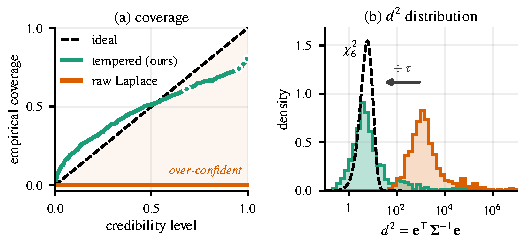
\includegraphics[width=\columnwidth]{fig3_calibration.pdf}
\caption{Measured calibration diagnostics (pooled test queries). (a) Coverage reliability: empirical coverage vs.\ credibility level under $\chi^2_6$; the raw Laplace covariance is severely overconfident (near-zero coverage) and the held-out temperature recovers most of the diagonal. (b) Sparsification: removing queries ranked by \emph{predicted} uncertainty tracks the oracle (rank by true error); AUSE is the area between.}
\label{fig:calib}
\end{figure}

\begin{figure}[t]
\centering
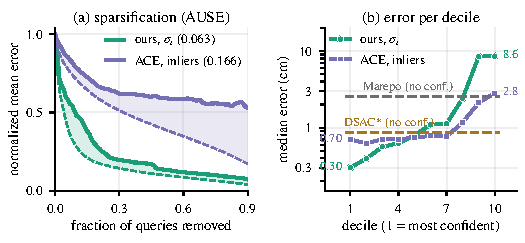
\includegraphics[width=\columnwidth]{fig5_uncertainty.pdf}
\caption{Uncertainty quality against ACE~\cite{ace} on identical queries (700 total). (a) Sparsification by each method's \emph{own} confidence signal, each curve normalized by its own initial error so that only ordering quality is compared. Ours tracks the oracle; the inlier count saturates. (b) Median error within each decile of reported confidence. A useful signal is monotone and wide-ranging.}
\label{fig:unc}
\end{figure}

\begin{figure}[t]
\centering
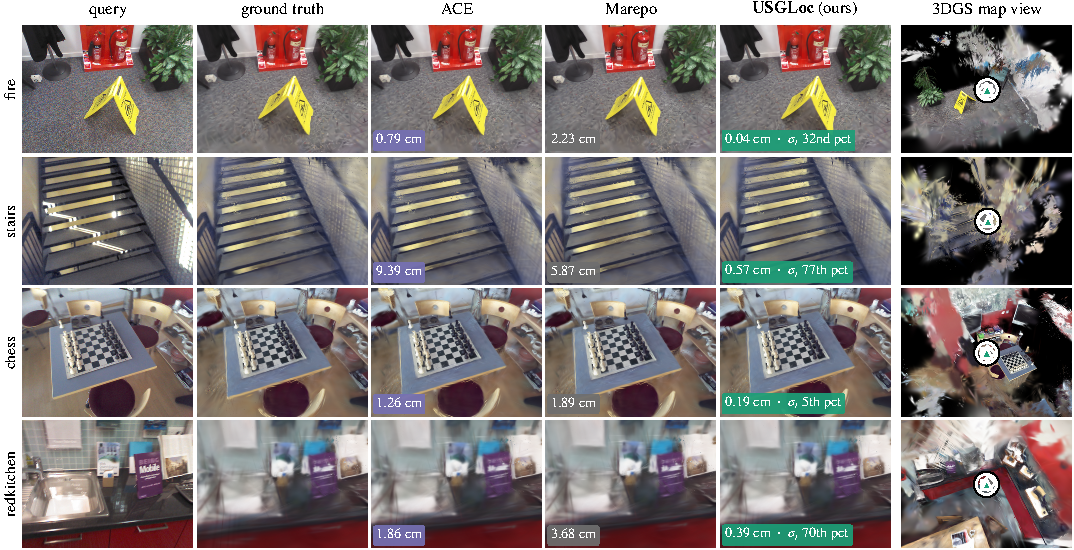
\includegraphics[width=\columnwidth]{fig_qual3.pdf}
\caption{Map rendered at the pose returned by \method{}, ACE and Marepo on identical queries, against ground truth. Rows are chosen by a fixed rule, one scene each: we are confident and right; we are wrong and say so; ACE fails where we do not; ACE beats us. Per-panel: translation error, and for \method{} the percentile of its own reported $\sigma_t$.}
\label{fig:qual3}
\end{figure}

\newcommand{\fpanel}[1]{\includegraphics[width=0.19\columnwidth]{fig4/#1}}
\begin{figure}[t]
\centering
\setlength{\tabcolsep}{1pt}
\begin{tabular}{ccccc}
\fpanel{a_query.png} & \fpanel{a_init.png} & \fpanel{a_refined.png} & \fpanel{a_vacuity.png} & \fpanel{a_weight.png}\\
\fpanel{b_query.png} & \fpanel{b_init.png} & \fpanel{b_refined.png} & \fpanel{b_vacuity.png} & \fpanel{b_weight.png}\\
{\scriptsize query} & {\scriptsize render @ $T_0$} & {\scriptsize render @ $\hat{T}$} & {\scriptsize vacuity $U_r$} & {\scriptsize weight $w$}\\
\end{tabular}
\caption{Qualitative results on two Chess test queries (seq-03/909 and seq-05/454; final error 0.27\,cm/0.13$^\circ$ and 0.37\,cm/0.17$^\circ$). Left to right: query image, render at the retrieved coarse pose $T_0$, render at the refined pose $\hat{T}$, rendered vacuity $U_r$ (bright = vacuous), and the per-pixel weight $w=e^{-\gamma U_r}$ that down-weights vacuous content in the refinement residual.}
\label{fig:qual}
\end{figure}

\begin{table}[t]
\centering
\caption{Calibration on 7Scenes, pooled over all 700 test queries (tempered). Coverage should match the nominal level; AUSE/ECE lower is better. The raw (untempered) Laplace covariance is severely overconfident.}
\label{tab:calib}
\setlength{\tabcolsep}{4pt}
\footnotesize
\begin{tabular}{lccccc}
\toprule
 & Cov.\,$68$ & Cov.\,$95$ & Cov.\,$99.7$ & AUSE\,$\downarrow$ & ECE\,$\downarrow$\\
Method & (\%) & (\%) & (\%) & (t) & \\
\midrule
Ideal $\chi^2$ ref.        & 68.3 & 95.4 & 99.7 & --   & --  \\
Raw Laplace (no $\tau$)    & 0.0  & 0.0  & 0.0  & 0.061 & 0.505 \\
\quad $-$ matching correction & 31.6 & 39.9 & 44.6 & 0.112 & 0.252\\
\textbf{\method{} (Ours)}  & \textbf{61.1} & \textbf{74.1} & \textbf{80.4} & \textbf{0.063} & \textbf{0.097} \\
\bottomrule
\end{tabular}
\end{table}

\subsection{Robustness}
\label{sec:robust}
We stress the map on Chess by fitting from fewer frames (every 40th and 80th instead of every 10th) and by distilling semantics from fewer frames (every 80th and 200th instead of every 20th). Accuracy degrades gracefully (measured on the Chess map before the fine-tune of Sec.~\ref{sec:setup}): the median moves from 0.56 to 0.78 and 0.65\,cm under the sparser fits and to 0.63 and 0.54\,cm under sparser distillation, all within a factor of 1.4, while the covariance temperature keeps coverage at the 95.4\% level between 83 and 89\% in every case against 79\% for the full map. The uncertainty is not merely inherited from a good map; it holds as the map gets worse, which is the property a deployed system needs.

\subsection{Ablation Study}
Table~\ref{tab:ablation} removes one component at a time on the easiest and the hardest scene. Stairs errors are bimodal (about 60\% of queries near 1.8\,cm, the rest mostly beyond 25\,cm with a failure median of 31\,cm), so its median is a threshold statistic and must be read next to the success rate. Three facts organize the table. First, the matching correction dominates everything else: without it the medians are 13.6 and 45.1\,cm, and every other row is a second-order effect on top of a working correction. Second, the components that matter are the ones that act \emph{after} the correction. On Stairs the vacuity pixel weight of \eqref{eq:refine} is worth 28\% (3.93 to 2.83\,cm), the inlier-based mixture weights of \eqref{eq:weights} are worth $2.1\times$ over the retrieval-prior weights, and reporting the mode rather than the mixture mean is worth $4\times$. Keeping $K{=}3$ hypotheses instead of one costs nothing in accuracy on Chess but is what makes the uncertainty informative: with $K{=}1$ the translation AUSE degrades from 0.056 to 0.373 on Chess and from 0.291 to 0.656 on Stairs, because a single Laplace covariance cannot represent an ambiguous scene. Third, and we state it plainly, two of the four evidential injection points are within run noise once the correction is in place: removing the correspondence gate or the instance gate changes the Stairs median by 0.07\,cm. The evidential channel earns its keep through the pixel weight and the mixture, not through the gates. Dempster and Yager fusion are indistinguishable here. Skipping photometric refinement entirely (snap only) trades 0.06--0.7\,cm of accuracy for markedly better coverage on Stairs (54/57 against 38/47), which is the accuracy--calibration trade-off a deployment can choose. On matched maps (same fitting recipe, only the head and its opinions differ) the softmax head is worse on both scenes: 0.62 against 0.56\,cm on Chess, and on Stairs it raises the share of failures beyond 5\,cm from 42\% to 56\%, which moves the median across the bimodal gap from 2.83 to 11.60\,cm while the successful queries are unchanged (1.8\,cm); AUSE is higher on both. The head comparison is only meaningful when the map recipe is held fixed, which the softmax map of our earlier grid did not satisfy.

\begin{table}[t]
\centering
\caption{Ablation on Chess and Stairs (seed 0, 100 queries): median translation error (cm), success rate at 5\,cm/5$^\circ$ (\%), and translation AUSE. Each row removes or replaces one component of the full method.}
\label{tab:ablation}
\setlength{\tabcolsep}{3pt}
\scriptsize
\begin{tabular}{@{}lcccccc@{}}
\toprule
& \multicolumn{3}{c}{Chess} & \multicolumn{3}{c}{Stairs} \\
\cmidrule(lr){2-4}\cmidrule(lr){5-7}
Variant & med. & SR & AUSE & med. & SR & AUSE \\
\midrule
Final (fine-tuned maps, agreement)      & 0.47 & 89 & 0.058 & 2.40 & 56 & 0.297 \\
Full, previous maps                     & 0.56 & 88 & 0.056 & 2.83 & 58 & 0.291 \\
\quad $-$ matching correction \eqref{eq:correction} & 13.55 & 39 & 0.068 & 45.08 & 6 & 0.220 \\
\quad $-$ correspondence gate           & 0.54 & 88 & 0.065 & 2.90 & 57 & 0.262 \\
\quad $-$ instance gate ($\lambda_u{=}0$) & 0.56 & 88 & 0.059 & 2.90 & 58 & 0.278 \\
\quad $-$ pixel weight ($\gamma{=}0$)   & 0.55 & 86 & 0.045 & 3.93 & 52 & 0.249 \\
\quad Dempster (no conflict)            & 0.55 & 88 & 0.056 & 2.79 & 58 & 0.287 \\
\quad retrieval-prior weights (pre-\eqref{eq:weights}) & 0.57 & 87 & 0.044 & 5.92 & 49 & 0.293 \\
\quad mixture mean instead of mode      & 0.55 & 87 & 0.052 & 11.30 & 30 & 0.184 \\
\quad point estimate ($K{=}1$)          & 0.56 & 87 & 0.373 & 4.04 & 51 & 0.656 \\
\quad snap only (no refinement)         & 0.62 & 92 & 0.077 & 3.54 & 54 & 0.229 \\
\quad softmax head, matched map          & 0.62 & 87 & 0.061 & 11.60 & 44 & 0.297 \\
\bottomrule
\end{tabular}
\end{table}

\subsection{Limitations}
Six limitations are worth stating. First, conflict handling is rule-bound: Dempster's rule suppresses conflict and Yager's routes it into vacuity, but neither models \emph{persistent} disagreement over time; a temporal conflict model could sharpen the dynamic-object signal. Second, each hypothesis's covariance is a local Laplace approximation, which is unimodal by construction; the mixture captures ambiguity across hypotheses, but heavy-tailed error within a basin is under-modeled, and coverage on repetitive scenes such as Stairs probes exactly this. Third, the evidential state inherits the failure modes of its frozen front end: content FastSAM does not segment, or CLIP cannot discriminate, earns vacuity rather than evidence, which is honest but reduces the usable signal. Fourth, the correction stage inherits the domain of its frozen matcher, and the final accuracy is bounded by the geometric fidelity of the 3DGS map itself: correcting from ground truth lands within 0.39\,cm on Chess but 1.01--1.24\,cm on Office and Stairs on the mapping-side frames used for map selection (0.47, 1.30 and 1.16\,cm on the test frames). Fifth, and most importantly for a reader weighing the method, \method{} is not the most accurate localizer available, and the reason is the map rather than the estimator: our correction cannot be more accurate than the geometry it registers against (Sec.~\ref{sec:correction}). Re-run with the authors' own solver, ACE~\cite{ace} is level in median error (pooled 0.87 versus 0.89\,cm) and fails less often (3\% versus 15\% of queries beyond 5\,cm); our remaining deficit is the Stairs failure tail and the two scenes with the highest map floors, Office and Pumpkin, on which we sit at the floor (extended report). The contribution is the calibrated distribution and the quality of its uncertainty, not state-of-the-art point accuracy. Sixth, coverage is still below nominal at high credibility levels, so the posterior remains over-confident in the tails. The evaluation is indoor and per-scene.

\subsection{Runtime}
On the RTX 5070 Ti, the median query takes 0.30\,s to encode (FastSAM + CLIP) and 6.3\,s to localize, pooled over all 700 test queries; per-scene medians range from 5.3 to 7.0\,s. The matching correction costs about 0.25\,s per hypothesis (2\,s for the top-8). The remainder is dominated by the per-hypothesis photometric refinement and its Laplace Jacobian, which reuses the refinement machinery. Map training takes 60--95\,s per scene at $320{\times}240$ and 140--370\,s for the four scenes fitted at $640{\times}480$. UGS-Loc reports 1.1\,s per refinement iteration with 8 particles and uses two iterations~\cite{ugsloc}; our budget is spent on $K{=}3$ full render-refinements, and reducing $K$ trades posterior richness for speed (Sec.~IV-E). With a single hypothesis ($K{=}1$) the median localization time falls to 5.9\,s on Chess and 4.0\,s on Stairs (from 6.0 and 6.9\,s), so the mixture costs roughly a factor of the number of components kept; per-stage timers are exposed in the released code.

%==============================================================================
\section{Conclusion}
We presented \method{}, a semantic 3D Gaussian Splatting localizer that returns a calibrated distribution over camera pose rather than a point. \method{} is built on one principle: the map's own uncertainty drives every stage of localization and survives to the output. A single evidential state is created when observations are encoded, and it is never discarded. It gates instance matching during retrieval. It gates the correspondences of the matching correction. It weights the rendering-refinement residual per pixel. It scales the Laplace covariance through a held-out temperature. These steps propagate uncertainty end-to-end into a Gaussian-mixture posterior on $SE(3)$. The posterior condenses to a single Gaussian for Bayesian filtering. Prior-free on 7Scenes, \method{} reaches 1.05\,cm/0.33$^\circ$ on average with a covariance whose ordering of its own errors approaches the oracle, and it is the only method in Table~\ref{tab:7scenes} that reports one. Future work includes a fully open-set semantic extension, tighter coupling with the navigation filter, learned (rather than Laplace) covariance heads, and on-board flight experiments on an indoor MAV.

%==============================================================================
% References live in references.bib (BibTeX, IEEEtran style).
% Compile: pdflatex -> bibtex -> pdflatex -> pdflatex (Overleaf does this for you).
\bibliographystyle{IEEEtran}
\bibliography{references}

\end{document}
